%% History:
% Pavel Tvrdik (26.12.2004)
%  + initial version for PhD Report
%
% Daniel Sykora (27.01.2005)
%
% Michal Valenta (3.12.2008)
% rada zmen ve formatovani (diky M. Duškovi, J. Holubovi a J. Žďárkovi)
% sjednoceni zdrojoveho kodu pro anglickou, ceskou, bakalarskou a diplomovou praci

\documentclass[12pt,twoside,a4paper]{book}   %two-page printing
\usepackage[czech]{babel}
\usepackage[T1]{fontenc} % pouzije EC fonty
\usepackage[utf8]{inputenc}
\usepackage{graphicx}
\usepackage{multirow}
%\usepackage{indentfirst} %1. odstavec jako v cestine.


\usepackage{k336_thesis_macros} % specialni makra pro formatovani DP a BP
 % muzete si vytvorit i sva vlastni v souboru k336_thesis_macros.sty
 % najdete  radu jednoduchych definic, ktere zde ani nejsou pouzity
 % napriklad: 
 % \newcommand{\bfig}{\begin{figure}\begin{center}}
 % \newcommand{\efig}{\end{center}\end{figure}}
 % umoznuje pouzit prikaz \bfig namisto \begin{figure}\begin{center} atd.


%%%%%%%%%%%%%%%%%%%%%%%%%%%%%%%%%%%%%
% Zvolte jednu z moznosti 
% Choose one of the following options
%%%%%%%%%%%%%%%%%%%%%%%%%%%%%%%%%%%%%
\newcommand\TypeOfWork{Diplomová práca} \typeout{Diplomova prace}
% \newcommand\TypeOfWork{Master's Thesis}   \typeout{Master's Thesis} 
% \newcommand\TypeOfWork{Bakalářská práce}  \typeout{Bakalarska prace}
% \newcommand\TypeOfWork{Bachelor's Project}  \typeout{Bachelor's Project}


%%%%%%%%%%%%%%%%%%%%%%%%%%%%%%%%%%%%%
% Zvolte jednu z moznosti 
% Choose one of the following options
%%%%%%%%%%%%%%%%%%%%%%%%%%%%%%%%%%%%%
% nabidky jsou z: http://www.fel.cvut.cz/cz/education/bk/prehled.html

%\newcommand\StudProgram{Elektrotechnika a informatika, dobíhající, Bakalářský}
%\newcommand\StudProgram{Elektrotechnika a informatika, dobíhající, Magisterský}
% \newcommand\StudProgram{Elektrotechnika a informatika, strukturovaný, Bakalářský}
 \newcommand\StudProgram{Elektrotechnika a informatika, strukturovaný, Navazující magisterský}
% \newcommand\StudProgram{Softwarové technologie a management, Bakalářský}
% English study:
% \newcommand\StudProgram{Electrical Engineering and Information Technology}  % bachelor programe
% \newcommand\StudProgram{Electrical Engineering and Information Technology}  %master program


%%%%%%%%%%%%%%%%%%%%%%%%%%%%%%%%%%%%%
% Zvolte jednu z moznosti 
% Choose one of the following options
%%%%%%%%%%%%%%%%%%%%%%%%%%%%%%%%%%%%%
% nabidky jsou z: http://www.fel.cvut.cz/cz/education/bk/prehled.html

%\newcommand\StudBranch{Výpočetní technika}   % pro program EaI bak. (dobihajici i strukt.)
\newcommand\StudBranch{Výpočetní technika}   % pro prgoram EaI mag. (dobihajici i strukt.)
%\newcommand\StudBranch{Softwarové inženýrství}            %pro STM
%\newcommand\StudBranch{Web a multimedia}                  % pro STM
%\newcommand\StudBranch{Computer Engineering}              % bachelor programe
%\newcommand\StudBranch{Computer Science and Engineering}  % master programe


%%%%%%%%%%%%%%%%%%%%%%%%%%%%%%%%%%%%%%%%%%%%
% Vyplnte nazev prace, autora a vedouciho
% Set up Work Title, Author and Supervisor
%%%%%%%%%%%%%%%%%%%%%%%%%%%%%%%%%%%%%%%%%%%%

\newcommand\WorkTitle{Model siete ZigBee}
\newcommand\FirstandFamilyName{Bc. Bernard Halás}
\newcommand\Supervisor{doc. Ing. Jan Janeček, CSc}


% Pouzijete-li pdflatex, tak je prijemne, kdyz bude mit vase prace
% funkcni odkazy i v pdf formatu
\usepackage[
pdftitle={\WorkTitle},
pdfauthor={\FirstandFamilyName},
bookmarks=true,
colorlinks=true,
breaklinks=true,
urlcolor=red,
citecolor=blue,
linkcolor=blue,
unicode=true,
]
{hyperref}




\begin{document}

%%%%%%%%%%%%%%%%%%%%%%%%%%%%%%%%%%%%%
% Zvolte jednu z moznosti 
% Choose one of the following options
%%%%%%%%%%%%%%%%%%%%%%%%%%%%%%%%%%%%%

%\selectlanguage{english} 

% prikaz \typeout vypise vyse uvedena nastaveni v prikazovem okne
% pro pohodlne ladeni prace



\typeout{************************************************}
\typeout{Zvoleny jazyk: cestina}
\typeout{Typ prace: \TypeOfWork}
\typeout{Studijni program: \StudProgram}
\typeout{Obor: \StudBranch}
\typeout{Jmeno: \FirstandFamilyName}
\typeout{Nazev prace: \WorkTitle}
\typeout{Vedouci prace: \Supervisor}
\typeout{***************************************************}
\newcommand\Department{Katedra počítačů}
\newcommand\Faculty{Fakulta elektrotechnická}
\newcommand\University{České vysoké učení technické v Praze}
\newcommand\labelSupervisor{Vedúci práce}
\newcommand\labelStudProgram{Študíjny program}
\newcommand\labelStudBranch{Obor}





%%%%%%%%%%%%%%%%%%%%%%%%%%    Poznamky ke kompletaci prace
% Nasledujici pasaz uzavrenou v {} ve sve praci samozrejme 
% zakomentujte nebo odstrante. 
% Ve vysledne svazane praci bude nahrazena skutecnym 
% oficialnim zadanim vasi prace.

%%%%%%%%%%%%%%%%%%%%%%%%%%    Titulni stranka / Title page 

\coverpagestarts

%%%%%%%%%%%%%%%%%%%%%%%%%%%    Podekovani / Acknowledgements 

\acknowledgements
\noindent
Rád by som sa poďakoval pánu Janečkovi za konzultácie, pripomienky a návrhy, ktoré mi ochotne poskytol počas vypracovávania tejto práce. Takisto vďaka patrí aj mojej rodine za podporu počas celého obdobia môjho štúdia.


%%%%%%%%%%%%%%%%%%%%%%%%%%%   Prohlaseni / Declaration 

\declaration{V Prahe dňa 21.\,5.\,2009}
%\declaration{In Kořenovice nad Bečvárkou on May 15, 2008}


%%%%%%%%%%%%%%%%%%%%%%%%%%%%    Abstract 
 
\abstractpage

This work describes a design of a LR-WPAN network model based on the ZigBee standard using OMNeT++, a popular discrete-event simulating engine. The text covers and evaluates the possibilities given by the addons for wireless and mobile networks modelling. The aim is to present one of many approaches based on the exact translation of the internal processes defined by the standards into the thorough structure of the model. This offers a clear view inside the model and sets a solid starting point for the future work on the product.

% Prace v cestine musi krome abstraktu v anglictine obsahovat i
% abstrakt v cestine.
\vglue60mm

\noindent{\Huge \textbf{Abstrakt}}
\vspace{8ex}

\noindent
Táto práca pojednáva o príprave modelu LR-WPAN siete postavenej na štandarde Zig\-Bee v populárnom simulačnom nástroji OMNeT++. Spracováva a vyhodnocuje možnosti ponúkané doplnkovými rozšíreniami k danému simulátoru pre modelovanie bezdrôtových a mobilných sietí. Práca si dáva za cieľ ponúknuť jeden z možných prístupov založený na presnom premietnutí procesov definovaných v špecifikácii aj do vnútornej štruktúry produktu, čím sa snaží o prehľadnosť a o poskytnutie solídneho odrazového bodu pre prípadné rozširovanie, alebo aktualizáciu modelu.

\noindent

%%%%%%%%%%%%%%%%%%%%%%%%%%%%%%%%  Obsah / Table of Contents 

\tableofcontents


%%%%%%%%%%%%%%%%%%%%%%%%%%%%%%%  Seznam obrazku / List of Figures 

\listoffigures


%%%%%%%%%%%%%%%%%%%%%%%%%%%%%%%  Seznam tabulek / List of Tables

\listoftables


%**************************************************************

\mainbodystarts
% horizontalní mezera mezi dvema odstavci
%\parskip=5pt
%JZ 11.12.2008 parskip bez tolerance? To neni rozumne, myslel jsem, ze sazime v TeXu, ne ve Wordu!
\parskip=5pt plus 4pt minus 4pt
% odstazeni prvniho radku odstavce (neaplikuje se na prvni odstace 
% kapitol, sekci, podsekci atd.)
%\parindent=10pt
%JZ 11.12.2008 -- indent v zavislosti na base font, proc 10pt?
\parindent=1.5em
% pokud chcete selektivne zamezit odsazeni 1. radku nektereho odstavce
% pouzijte prikaz \noindent.

%**************************************************************

% Pro snadnejsi praci s vetsimi texty je rozumne tyto rozdelit
% do samostatnych souboru nejlepe dle kapitol a tyto potom vkladat
% pomoci prikazu \include{jmeno_souboru.tex} nebo \include{jmeno_souboru}.
% Napr.:
% \include{1_uvod}
% \include{2_teorie}
% atd...

%*****************************************************************************
\cleardoublepage\chapter{Úvod}

\indent\indent Od napísania mojej prvej práce zaoberajúcej sa simuláciami senzorových sietí~\cite{halas03} uplynuli približne tri roky. Technológia sa posunula o malý krok vpred a zariadenia pre komunikáciu v senzorových sieťach nenáročných na šírku datového prenosu sa stávajú cenovo dostupnejšie. Vynárajú sa otázky, či pri masívnejších nasadeniach sú tieto siete schopné vykonávať požadované úlohy pri zdieľaní prenosového média spolu s takisto čoraz rozšírenejšími technológiami bezdrôtových sietí ako Wi-Fi$^{TM}$, alebo Bluetooth$^{TM}$, s ktorými zdieľajú časti frekvenčného spektra pre svoju komunikáciu.\\
\indent Na základe týchto skutočností sa ponúkalo zúročiť získané skúsenosti so simulačnými systémami a pripraviť aktuálnejší model siete ZigBee postavenej nad technológiou IEEE 802.15.4$^{TM}$, ktorý by reflektoval zmeny štandardov z uplynulých mesiacov a rokov a ktorý by ponúkal bohatšie možnosti simulácii s výsledkami bližšími reálnemu svetu.

\cleardoublepage\chapter{Špecifikácia požiadaviek na navrhovaný systém}

\section{Popis problému}
\indent\indent Špecifikácia siete ZigBee~\cite{zigbee08} predstavuje uzavretý dokument popisujúci udalosti, procesy a obsah komunikácie medzi jednotlivými modulmi v rámci hierarchie definovanej takisto týmto dokumentom. Štandard ZigBee hovorí o vyšších sieťových vrstvách. Vynecháva fyzickú a linkovú vrstvu. V daných prípadoch sa spolieha na iný dokument, na špecifikáciu protokolu IEEE 802.15.4\texttrademark~\cite{ieee06}.\\
\indent\indent Informácie obsiahnuté v týchto dvoch dokumentoch je nutné premietnuť do vnú\-tornej štruktúry modelov simulátora pre získanie čo najvernejších výsledkov. Od modelu sa takisto očakáva reflektovanie nárokov vkladaných do reálnych sietí, a to mobilita daných prvkov, ktorá nie je bezdrôtovým senzorových sietí cudzia a určite zakomponovanie javov sprevádzajúcich šírenie elektromagnetického signálu vzduchom. Z experimentálnej stránky veci nás zaujíma aj možnosť nasadenia technológie TCP/IP nad technológiami ZigBee/IEEE 802.15.4

\section{Požiadavky na model}
\indent\indent Požiadavky kladené na simulačný model by sa dali zhrnúť do nasledujúcich niekoľko bodov:
\begin{enumerate}
  \item Obsiahnutie základných vlastností deklarovaných v štandardoch ZigBee a IEEE 802.15.4
  \item Podpora mobility všetkých sieťových prvkov
  \item Zahrnutie vplyvov prostredia (interferencia, šum, ...)
  \item Pripraviť rozhranie umožňujúce prenos IP (Internet Protocol) paketov
  \item Modularita pre ľahké aktualizácie modelu v prípade vydania nových verzii štandardov
  \item Výpočtová náročnosť vykonávaných simulácii v rozumných medziach
\end{enumerate}
\subsection{Vlastnosti sietí postavených na IEEE 802.15.4}
\indent\indent Štandard uvedený technickej verejnosti v roku 2003 špecifikuje fyzickú a linkovú vrstvu Low-Rate WPAN (Wireless Personal Area Network) sietí. Charakteristické vlastnosti týchto sietí sú nízka spotreba, nízka dátová priepustnosť, v prípade potreby garancia istého prenosového pásma a jednoduchosť jednotlivých procesov, z ktorej vyplývajú nevysoké požiadavky na riadiace procesory. Typická aktivita v čase zariadení tohoto typu je pod 0.1\%. Elementy, ktoré sú pri takto nastavených požiadavkách na sieť potrebné pre jej efektívne fungovanie a bez ktorých sa náš simulačný model nezaobíde sú nasledovné:
\begin{description}
  \item[RFD/FFD prvky] (Full Functionality Device, Reduced Functionality Device) prvky siete IEEE sa podľa funkčnosti delia na dve hlavné skupiny. Konštrukčne jednoduchšie označujeme ako RFD. V teórii grafov by sme ich vďaka ich polohe v stromovej topológii označili listami. Odpoveď na to, prečo potrebujeme zložité (FFD) a jednoduché prvky (RFD) je v tom, že v rámci stromovej hierarchie len tie zariadenia nachádzajúce sa vyššie majú svoju úlohu doplnenú o posielanie beacon rámcov, smerovanie paketov, prijímanie žiadostí o asociáciu siete a pod.
  \item[Beacon rámce] sú rámce vysielané v pravidelných intervaloch zariadením typu FFD a majú za úlohu informovať o plánovaných dátových prenosoch, topológii a~o~konfiguračných premenných danej siete. Tieto rámce sa objavujú pravidelne a vďaka tomu príjemca vie, kedy si môže dovoliť vypnúť prijímač mikrovlnného signálu s cieľom šetriť energiu s istotou nepremeškania žiadneho beacon rámca.
  \item[CSMA-CA] (Carrier Sense Multiple Access - Collision Avoidance) je metóda prístupu k zdieľanému médiu. V našom prípade je médiom vzduch a metóda nám pomáha vyvarovať sa kolízii rámcov pri ich vysielaní a príjme.
  \item[GTS mechanizmus] (Guaranteed Time Slot) je systém periodického rezervovania časových slotov pre posielanie rámcov medzi prvkami v stromovej topológii. Môže byť v prípade potreby zárukou získania určitej šírky prenosového pásma pre jednotlivé sieťové prvky, a~teda umožňovať komunikáciu s nízkou latenciou.
 \end{description}
\indent\indent O týchto vlastnostiach a o spôsobe ich prípadnej implementácie si povieme viac v neskorších kapitolách.
\subsubsection{Mobilita}
\indent\indent Na sieťové prvky bezdrôtových sietí je často kladený požiadavok mobility daného prvku v priestore, ktorý je v konečnom dôsledku premietaný do úprav pozície daného prvku v topológii siete. Pre simulátor teda vyplýva, že musí dynamicky v čase vedieť polohu prvku pre výpočet hodnôt fyzikálnych veličín charakterizujúcich prenos a následný príjem signálu.\\
\indent Čo sa týka daného modelu, ten by mal mať schopnosť reagovať v prípade, že komunikačné cesty po zmene polohy už nie sú schopné dostatočne kvalitne prenášať rámce. Toto je vlastnosť prvkov, na ktorú sa v špecifikácii~\cite{ieee06} myslí, a teda vo finálnom modeli bude zahrnutá.
\subsubsection{Vlastnosti prenosového média}
\indent\indent Siete, ktoré sú predmetom nášho záujmu, pristupujú k zdieľanému médiu - vzduchu. Tým, že médium je spoločné pre všetky prvky siete, stav, v ktorom sa nachádza, má rôznou mierou vplyv na všetky prijímače elektromagnetického signálu. Mnohé simulátory sa zameriavajú práve na verné spracovanie tejto skutočnosti. Ich metódy napríklad pre výpočet prijímaného výkonu, alebo odstupu signálu od šumu (SNR) sú výborne spracované a budú pre náš simulátor užitočné.
\subsection{Modularita návrhu}
\indent\indent Podobne ako v predchádzajúcej práci~\cite{halas03} sa nám overil diferencovaný prístup k jednotlivým vrstvám  odvodený od OSI-ISO modelu, tiež teraz budú jednotlivé sieťové prvky zložené z viacerých modulov, ktoré budú medzi sebou komunikovať ideálne len predávaním správ.\\
\indent Tento pohľad na komplexnú štruktúru sieťových prvkov nám zaručí jednoduchosť prípadných neskorších zásahov napríklad z dôvodu úprav v smerovacích mechanizmoch. V danom prípade bude nutné iba vykonať zmeny v module, ktorý zabezpečuje smerovanie paketov.


\cleardoublepage\chapter{Zigbee a IEEE 802.15.4}

\indent\indent S nástupom zariadení pre bezdrôtovú komunikáciu určených pre použitie v lokálnych (LAN - Local Area Network), alebo osobných (PAN - Personal Area Network) sieťach sa začala vynárať možnosť využiť bezdrôtovú technológiu aj pre inteligentné systémy, ktoré nevyžadujú vysoké prenosové rýchlosti. To bol popud pre vznik štandardu pre bezdrôtovú komunikáciu v LAN a PAN sieťach charakteristickú nízkymi prenosovými rýchlosťami, malými nárokmi na konfiguráciu a aj samotnú prevádzku.\\

\section{IEEE 802.15.4}
\indent\indent Tento štandard definujúci fyzickú (PHY - Physical) a linkovú (MAC - Media Access Control) vrstvu bol prvý krát predstavený v roku 2003~\cite{ieee03}. Od toho momentu je ďalej vyvíjaný dvoma smermi. Jeden bol predstavený v roku 2006 pod označením IEEE 802.15.4b~\cite{ieee06}, formálne aj označovaný ako IEEE 802.15.4b-2006 vďaka roku svojho publikovania. Rozšíril možnosti modulácie signálu, a teda aj zvýšil maximálne prenosové rýchlosti vo frekvenčných pásmach 868/915~MHz. Umožnenie viacerých druhov modulácie v týchto prenosových pásmach umožnilo zjednodušenie samotných zariadení, pretože na komunikáciu v 868/915~MHz a 2.4 GHz už stačil iba jeden modulačný čip. Druhú vetvu vývoja prestavoval štandard označovaný ako IEEE 802.15.4a prípadne formálne IEEE 802.15.4a-2007, ktorý operuje v pásme Ultra-Wideband (UWB). Týmto sa však nebudeme v tejto práci zaoberať. Všetky nasledovné informácie sa budú viazať k verzii IEEE 802.15.4b-2006, ak nebude uvedené inak.\\
\indent Siete postavené podľa IEEE 802.15.4b-2006 sú charakteristické tým, že ponúkajú
\begin{itemize}
\item Prevádzku v bezlicencovaných frekvenčných pásmach
\item Prenosové rýchlosti na úrovniach 250, 100, 40, alebo 20 kb/s
\item Topológiu v tvare hviezda (star), alebo každý s každým (peer-to-peer)
\item Komunikáciu pomocou 64-bitových, alebo 16-bitových adries
\item Mechanizmus alokácie časových slotov (GTS)
\item Prístup na médium vyhýbajúci sa kolíziám (CSMA-CA)
\item Spoľahlivý prenos dát s mechanizmom kotroly integrity (FCS - Frame Check Sequence) a potvrdzovaním dát
\item Aktivitu zariadení priemerne na úrovni 0.1\% doby cyklu
\end{itemize}
\indent Všeobecne, IEEE 802.15.4 predstavuje základ pre tzv. LR-WPAN (Low-Rate Wireless PAN) siete. Naň sa spoliehajú technológie ako WirelessHART, MiWi, alebo aj ZigBee.\\
\subsection{Topológia}
\indent\indent Pre vytvorenie PAN siete je potrebné, aby minimálne jeden z prvkov bol typu FFD. Tieto zariadenia majú schopnosť vytvárať WPAN sieť (v prípade, že fungujú aj ako PAN koordinátor), okrem toho aj prideľujú sieťové adresy, asociujú nové prvky do siete a vysielajú tzv. beacon rámce.\\
\indent Prvky FFD a RFD môžu tvoriť 2 druhy usporiadaní z pohľadu topológie siete - hviezdu a každý s každým.\\
\subsubsection{Hviezda (Star)}
\indent\indent Siete typu Hviezda fungujú na sebe nezávisle a bez problémov ich môže operovať viac vo svojom vzájomnom dosahu. Každá z nich musí byť ale jednoznačne identifikovateľná svojím PAN identifikátorom. V centre siete je PAN koordinátor. Zariadenie, či už FFD, alebo RFD si pri pripájaní do siete môže vybrať ľubovoľný PAN koordinátor vo svojom dosahu a požiadať ho o asociáciu. Príklad takejto siete je zobrazený na obrázku~\ref{fig:topology_star}.\\
\begin{figure}[htbp]
\begin{center}
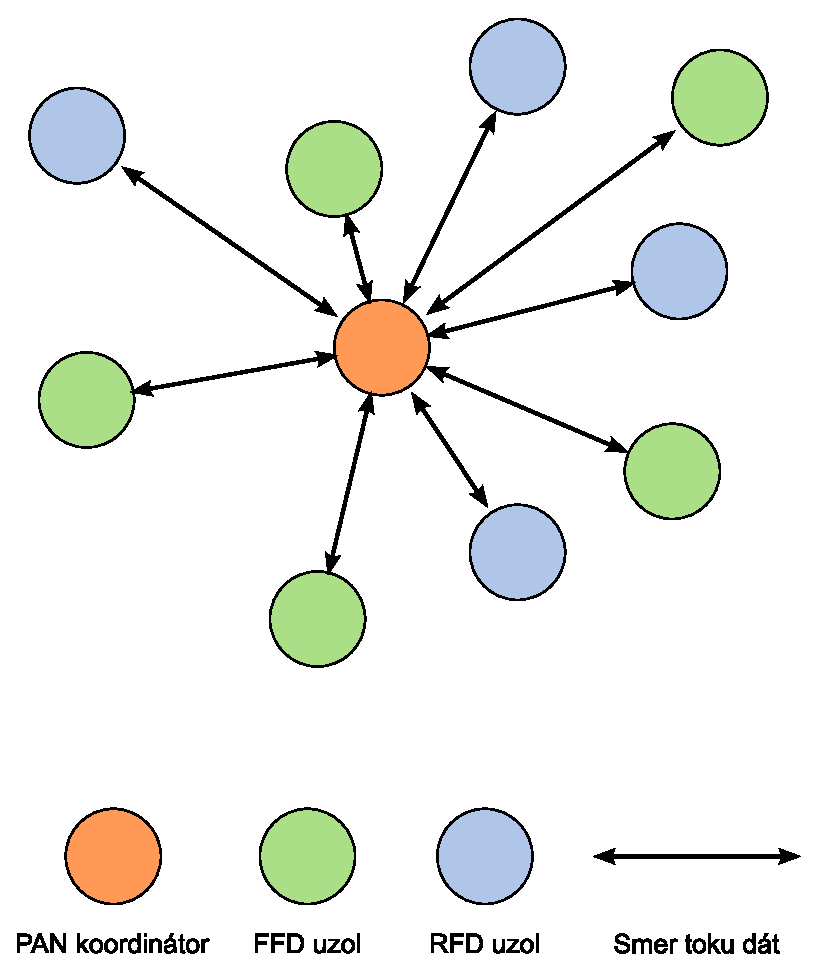
\includegraphics[width=120mm]{figures/topology_star}
\caption{Topológia typu hviezda}
\label{fig:topology_star}
\end{center}
\end{figure} 
\subsubsection{Každý s každým (Peer-to-Peer)}
\indent\indent V tomto type topológie je implementovaná ide aby mohlo každé zariadenie komunikovať s ľubovoľným iným vo svojom dosahu. Takisto v takýchto sieťach existuje jeden FFD prvok v roli PAN koordinátora. Ukážka na obrázku~\ref{fig:topology_p2p}.\\
\begin{figure}[htbp]
\begin{center}
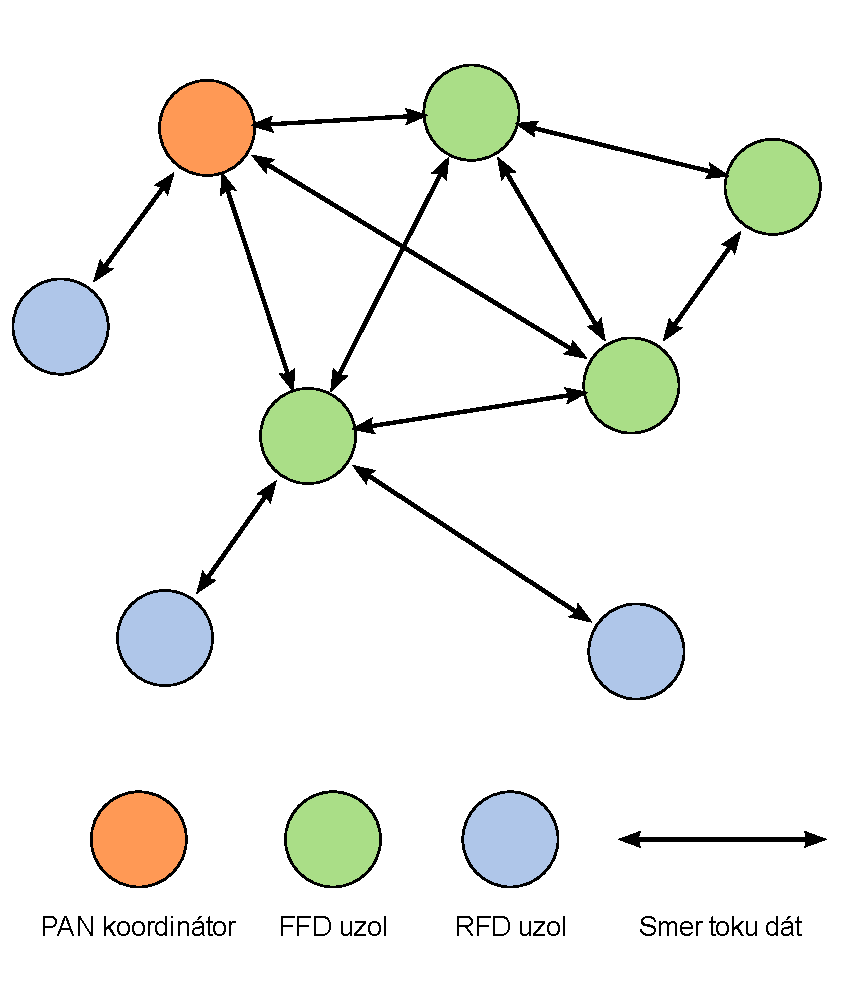
\includegraphics[width=120mm]{figures/topology_p2p}
\caption{Topológia typu každý s každým}
\label{fig:topology_p2p}
\end{center}
\end{figure} 
\indent Z tohoto typu sietí je odvodený variant Zhluk stromov (Cluster Tree). V takejto topológii je prevažná väčšina zariadení typu FFD. Zariadenia typu RFD sa pripájajú k~stromu ako listy. Všetky FFD sú schopné vysielať synchronizačné beacon rámce. Z~nich môže byť však len jeden PAN koordinátor. Ak bude asociácia zariadenia do siete z~nejakého dôvodu odmietnutá, prvok môže vyhľadať iné FFD zariadenie a skúsiť asociáciu u~neho.\\
\indent V prípade, že sú splnené určité podmienky, PAN koordinátor môže požiadať FFD prvok v rámci svojej siete, aby  zformoval novú PAN sieť s novým identifikátorom. Ostatné zariadenia sa potom môžu pripájať až budú tvoriť podobné štruktúry, ako je tá na obr.~\ref{fig:topology_cluster}. Volá sa zhluk stromov (Cluster Tree) Takáto konfigurácia ponúka plošne široké pokrytie, na druhú stranu však správy pri prechode cez viaceré PAN zvyšujú svoju latenciu.\\
\begin{figure}[htbp]
\begin{center}
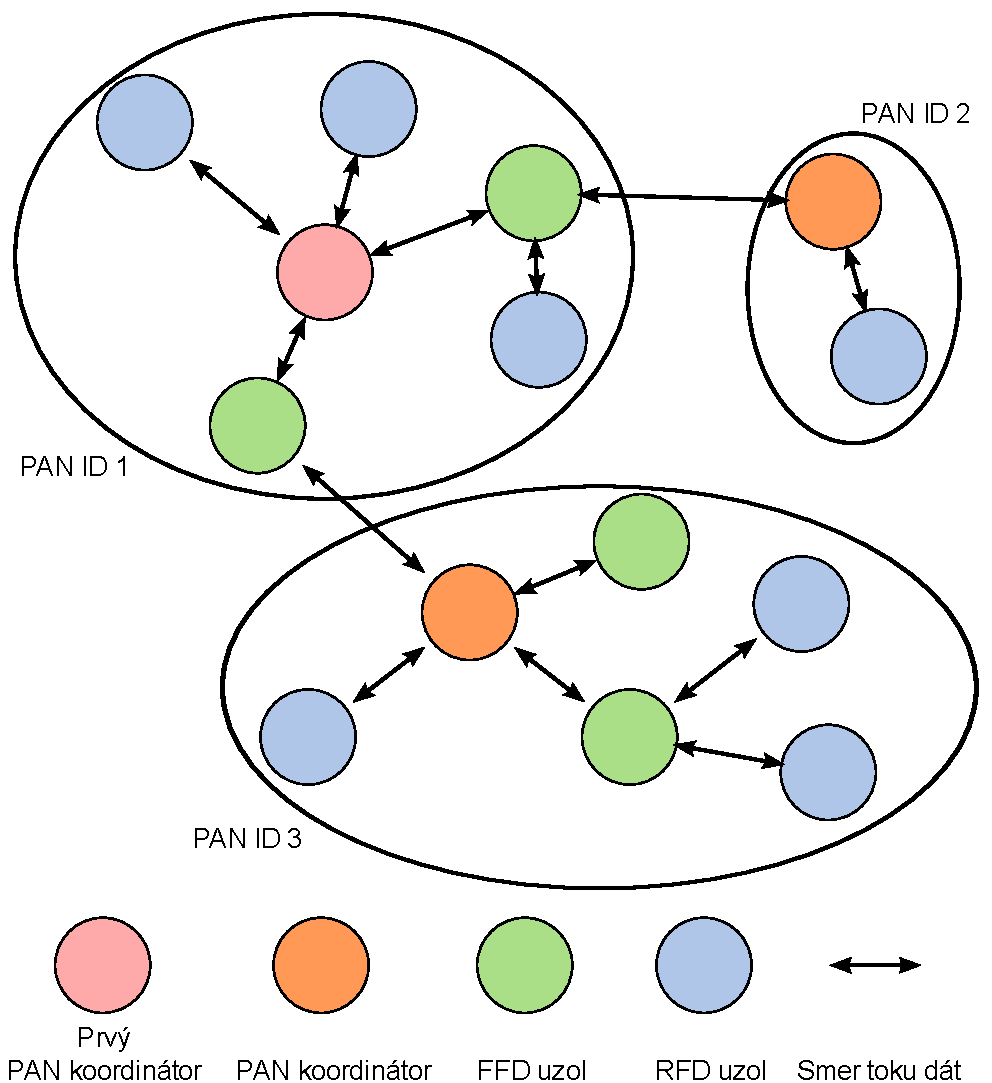
\includegraphics[width=120mm]{figures/topology_cluster}
\caption{Topológia typu zhluk stromov}
\label{fig:topology_cluster}
\end{center}
\end{figure} 
\subsection{Fyzická vrstva}
\indent\indent Ako už bolo spomenuté, jedná sa o technológiu pracujúcu so vzduchom ako zdieľaným médiom. Frekvenčné pásma, v ktorých zariadenia operujú, sú uvedené v tabuľke~\ref{tab:frequencies}. Je vhodné podotknúť, že sa jedná o tzv. bezlicencované (ISM - Industrial Scientific and Medical) pásma, avšak kým 2.4 GHz je s malými obmedzeniami k dispozícii takmer po celom svete, pásmo ISM 868~MHz je len v Európe a ISM 902-928~MHz je k dispozícii len v USA.\\
\begin{table}[htbp]
\begin{center}
\begin{tabular}{|c|c|l|c|c|l|}
  \hline
  \multirow{2}{*}{\textbf{PHY}} & \multirow{2}{*}{\textbf{Frekvencia}} & \multirow{3}{*}{\textbf{Modulácia}} & \textbf{Prenosová} & \textbf{Symbol} & \multirow{3}{*}{\textbf{Symboly}} \\ 
  \multirow{2}{*}{(MHz)} & \multirow{2}{*}{(MHz)} & & \textbf{rýchlosť} & \textbf{rate} & \\ 
  & & & (kbps) & (ksym/s) & \\ [0.5ex]
  \hline\hline
  \multirow{2}{*}{868/915} & 868--868.6 & BPSK & 20 & 40 & Binárne\\
  & 902--928 & BPSK & 40 & 40 & Binárne\\ [0.5ex]
  \hline
  \multirow{2}{*}{868/915} & 868--868.6 & ASK & 250 & 12.5 & 20-bitové PSSS\\
  & 902--928 & ASK & 250 & 50 & 5-bitové PSSS\\ [0.5ex]
  \hline
  \multirow{2}{*}{868/915} & 868--868.6 & O-QPSK & 100 & 25 & 16-kové ortogonálne\\
  & 902--928 & O-QPSK & 250 & 62.5 & 16-kové ortogonálne\\ [0.5ex]
  \hline
  2450 & 2400--2483.5 & O-QPSK & 250 & 62.5 & 16-kové ortogonálne\\ [0.5ex]
  \hline
\end{tabular}
\caption{Používané frekvenčné pásma, modulácie a kódové symboly}
\label{tab:frequencies}
\end{center}
\end{table}
\indent\indent Pre komunikáciu je vyhradených 27 kanálov, ktoré sú združené do troch tzv. stránok kanálov. Takýto spôsob členenia je z historických dôvodov a z dôvodov spätnej kompatibility so zariadeniami fungujúcimi na IEEE 802.15.4-2003. Stránky sú očíslované v rozsahu 0--31, pričom v aktuálne sú stránky 3--31 rezervované do budúcna.\\ 
\indent Na definovanie frekvencie, prenosovej rýchlosti a modulácie je nutné poznať kombináciu hodnoty stránky kanálu a označenie kanálu (z rozsahu 0--26). Pre určenie stránky kanálu je využitých horných 5 bitov (MSB - most significant bit). Pre označenie kanálu sa používa 27-bitová mapa. To znamená, že informácia definujúca potrebné parametre pre komunikáciu na úrovni fyzickej vrstvy sa kompletne obsiahne do 32-bitového identifikátora (viď obr.~\ref{fig:channel_page}). Jednotlivé kombinácie hodnôt stránky kanálov a samotného kanálu sú bližšie rozpísané v tabuľke~\ref{tab:channel_page}.\\
\indent Štandard počíta s tromi základnými typmi modulácie, BPSK (Binary Phase Shift Keying), ASK (Amplitude Shift Keying) a O-QPSK (Offset-Quadrature Phase Shift Keying). PSK (Phase Shift Keying) je modulačná schéma, ktorá transportuje dáta pomocou zmeny fázy referenčného signálu. Jej základná varianta BPSK pracuje s dvoma fázami posunutými o 180 stupňov. To znamená, že jeden kódový symbol reprezentuje jeden bit informácie. Tento spôsob modulácie je relatívne odolný voči rušeniu, ale vyžaduje zložitejšie vysielacie a prijímacie obvody. Hustota informácii na prenesený symbol je nízka, teda je skôr vhodnejší na komunikáciu pri nízkych prenosových rýchlostiach (v prípade 802.15.4 hovoríme o hodnotách 20 a 40 kbps). Alternatívu na frekvenčných pásmach 868/915~MHz predstavil štandard IEEE 802.15.4b-2006, a to použitie ASK modulácie, kedy dáta sú reprezentované variáciami v amplitúde prenášaného signálu. Fáza a frekvencia zostávajú konštantné. Jej princíp je jednoduchý, avšak je citlivá na rušenie, odrazy a pod. ASK nepredstavuje veľmi efektívny spôsob modulácie. Tretí použitý spôsob modulácie datových bitov na nosnú v štandarde IEEE 802.15.4 predstavuje varianta O-QPSK. Pôvodne bol tento typ modulačnej schémy myslený len pre 2.4~GHz ISM pásmo, ale uvedenie tohoto typu modulácie aj pre ostatné frekvenčné pásma, predstavené so štandardom IEEE 802.15.4b-2006, znamenalo zjednodušenie pre koncové prvky, pretože pre prácu v pásmach 868~MHz, 915~MHz a 2.4~GHz potom stačí jeden modulačný a demodulačný obvod. Schéma O-QPSK teda pracuje so štyrmi variáciami posunu fázy (4 stavy), to znamená, že vie na jeden symbol modulovať 2 bity ($2^{2}=4$). Identifikátor \textit{offset} v názve charakterizuje posun pri modulovaní párnych a nepárnych bitov. Tento posun má veľkosť, ktorá predstavuje polovicu dĺžky vysielania jedného symbolu. Dochádza k posunu fázy vždy len o 90 stupňov, čo zabraňuje skokovým zmenám amplitúdy. Táto \textit{offset} varianta kvadratúrnej fázovej modulácie je často preferovaná.\\
\begin{figure}[htbp]
\begin{center}
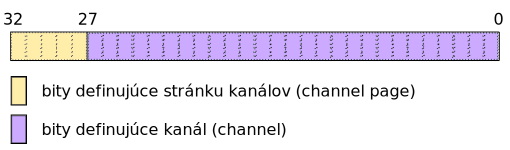
\includegraphics[width=120mm]{figures/channel_page}
\caption{32-bitový identifikátor kanálov a stránky kanálov}
\label{fig:channel_page}
\end{center}
\end{figure}
\begin{table}[htbp]
\begin{center}
\begin{tabular}{|c|c|c|c|c|}
  \hline
  \textbf{Stránka kanálu} & \textbf{Stránka kanálu} & \textbf{Číslo kanálu} & \textbf{Frekvenčné} & \\
  (dekadicky) & (binárne) & (dekadicky) & \textbf{pásmo} & \raisebox{1.5ex}{\textbf{Modulácia}} \\
  \hline
  \hline
  \multirow{3}{*}{0} & \multirow{3}{*}{0 0 0 0 0} & 0 & 868 MHz & BPSK \\
  \cline{3-5}
  & & 1--10 & 915 MHz & BPSK \\
  \cline{3-5}
  & & 11--26 &  2.4 GHz & O-QPSK \\ [0.5ex]
  \hline
  \multirow{3}{*}{1} & \multirow{3}{*}{0 0 0 0 1} & 0 & 868 MHz & ASK \\
  \cline{3-5}
  & & 1--10 & 915 MHz & ASK \\
  \cline{3-5}
  & & 11--26 & \multicolumn{2}{|c|}{Rezervované} \\ [0.5ex]
  \hline
  \multirow{3}{*}{2} & \multirow{3}{*}{0 0 0 1 0} & 0 & 868 MHz & O-QPSK \\
  \cline{3-5}
  & & 1--10 & 915 MHz & O-QPSK \\
  \cline{3-5}
  & & 11--26 & \multicolumn{2}{|c|}{Rezervované} \\ [0.5ex]
  \hline
  3--31 & 0 0 0 1 1 -- 1 1 1 1 1 & \multicolumn{3}{|c|}{Rezervované} \\ [0.5ex]
  \hline
\end{tabular}
\caption{Zoznam jednotlivých kombinácii kanálov, frekvenčných pásiem a použitých modulácii podľa nastavenia identifikátorov kanálov a stránky kanálov}
\label{tab:channel_page}
\end{center}
\end{table}
\subsection{Linková vrstva}
\indent\indent Linková vrstva IEEE 802.15.4b podľa~\cite{ieee06} je jednoduchá, ale flexibilná. Riadi a kontroluje prístup k zdieľanému médiu. K tomuto využíva nasledovné mechanizmy:
\begin{itemize}
\item Vysielanie beacon rámcov (periodicky, alebo neperiodicky v závislosti od aktuálnej konfigurácie siete)
\item Synchronizácia podľa beacon rámcov vysielaných svojimi susedmi
\item Podieľanie sa na procesoch asociácie a disasociácie v PAN sieti
\item V prípade požiadavku, podpora zabezpečenia
\item Prístup k médiu pomocou CSMA-CA algoritmu
\item Riadi a prideľuje GTS časové sloty 
\end{itemize}
\subsection{Beaconing a non-beaconing módy}
\indent\indent  Linková vrstva môže pracovať v dvoch základných režimoch - tzv. beaconing mód a~non-beaconing mód. Rozdiel medzi týmito módmi nie je v tom, či sú beacon rámce v~sieti posielané, ale v tom, či sú tieto rámce posielané pravidelne. V prípade, že je hodnota atribútu u koordinátora siete $macSuperframeOrder < macBeaconOrder$, to znamená, že sieť pracuje v beaconing móde a beacon rámce sú posielané pravidelne v~intervale vypočítanom podľa vzťahu 
$$ beaconPeriod = aBaseSuperframeDuration * 2^{macBeaconOrder}$$
kde výsledná hodnota intervalu je v symboloch. Podľa tabuľky~\ref{tab:frequencies} sa táto hodnota dá previesť na čas v sekundách. Hodnota konštanty aBaseSuperframeDuration je $960$ a~predstavuje dĺžku najkratšieho možného intervalu v symboloch oddeľujúceho začiatky dvoch beacon rámcov.\\
\indent Alternatívu predstavujú zhodné hodnoty atribútov \textit{macBeaconOrder} a \textit{macSuperframeOrder}. Vtedy sa jedná o non-beaconing mód a beacon rámce sa posielajú len ako odpoveď na explicitnú požiadavku o ich zaslanie.\\
\subsection{Superframe rámec}
\indent\indent Nami navrhovaný model uvažuje použitie beaconing módu, ktorý ponúka zaujímavejší mechanizmus komunikácie a využíva možnosti dané periodicitou v zasielaní riadiacich a kontrolných beacon rámcov. V tomto beaconing móde sa využíva komunikačná štruktúra, ktorá sa nazýva superframe rámec. Superframe rámec vymedzuje 4 periodicky sa opakujúce úseky (obr.~\ref{fig:superframe}) a pre každý z nich platia pravidlá pre posielanie a príjem dát. Superframe rámec vždy obsahuje 16 superframe slotov o dĺžke $aBaseSlotDuration * 2^{macSuperframeOrder}$ symbolov dynamicky distribuovaných do Contention Access periódy a Contention Free periódy. Slot, v ktorom je vysielaný beacon rámec je označovaný ako slot 0. Konštanta \textit{aBaseSlotDuration} má hodnotu $60$.\\
\begin{figure}[htbp]
\begin{center}
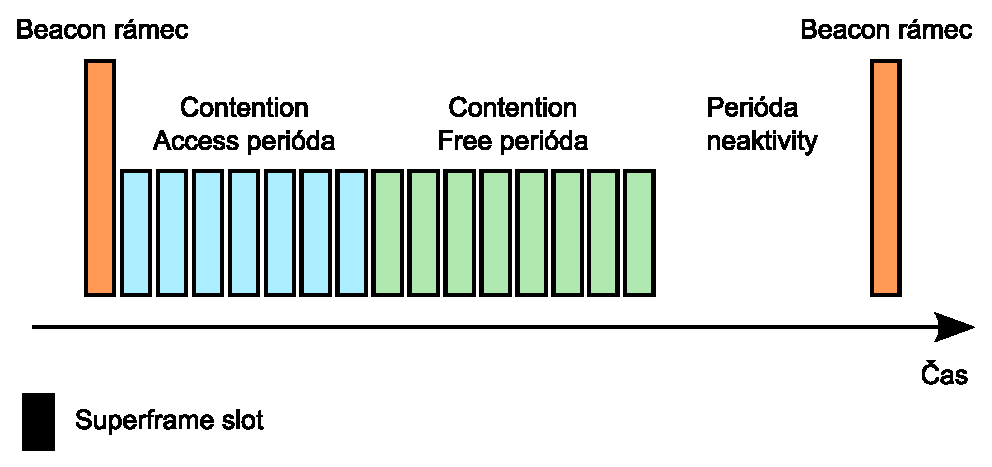
\includegraphics[width=140mm]{figures/superframe}
\caption{Štruktúra superframe rámca (obrázok nie je v mierke)}
\label{fig:superframe}
\end{center}
\end{figure}
\subsubsection{Beacon rámec}
\indent\indent Na úvod každého superframe rámca je FFD prvkom, ktorý je v sieti pripojený ako smerovač (router), posielaný beacon rámec. Obsahuje informačné polia, ktoré okrem iného obsahujú atribúty \textit{macBeaconOrder} a \textit{macSuperframeOrder} definujúce isté vlastnosti danej PAN siete. Z týchto polí vychádzajú hraničné časovače určujúce dĺžky jednotlivých úsekov superframe rámca. Okrem toho definuje aj koniec Contention Access periódy pomocou identifikátora \textit{FinalCAPSlot}.\\
\indent Beacon rámec je vysielaný prvkom bez použitia CSMA metódy, pretože všetky prvky v dosahu vysielača daného FFD prvku by sa mali synchronizovať na periodicitu týchto rámcov a nevysielať žiadne dáta na prenosové médium v čase, keď sa očakáva beacon rámec.\\
\paragraph{Contention Access perióda}
Počas tejto periódy prvky môžu pristupovať na médium pomocou metódy CSMA-CA. Tento moment slúži hlavne na vybavovanie žiadosti o asociáciu do siete, prípadne žiadosti o prenos užitočných dát smerom od FFD prvku. V takom prípade sú dáta, ktoré chce FFD poslať svojim susedom indikované v beacon rámci. FFD prvky majú väčšinou fronty na zasielanie týchto rámcov s užitočnými dátami pre koncové zariadenia. Ak si sused daného smerovača nevyžiada dáta po uplynutí nejakého konkrétneho počtu superframe rámcov od ich prvého indikovania v beacon rámci, smerovač ich z tejto fronty zahadzuje.\\
\indent Prvok, ktorému smerovač v beacon rámci neindikoval, že má pre neho vo svojich frontách zaradené dáta, a tento prvok ani nemá záujem žiadne dáta poslať smerom k~FFD zariadeniu môže vypnúť svoje vysielacie a prijímacie obvody a šetriť tak energiu.\\
\paragraph{Contention Free perióda}
Časový interval v ktorom sa prenášajú dáta pomocou mechanizmu GTS (Guaranteed Time Slot) sa nazýva Contention Free perióda. GTS mechanizmus alokuje určitý počet superframe slotov pre prenos dát, ktoré často majú periodický charakter. Beacon rámec posielaný smerovačom na úvod superframe rámca definuje aj počet alokovaných superframe slotov združených do GTS slotov a pre každý z týchto GTS slotov pomocou 16-bitovej, alebo 64-bitovej adresy určí druhú stranu komunikačného toku. Pomocou jednoduchej bitovej mapy je následne určený smer komunikácie (smerom od smerovača/smerom k smerovaču). GTS mechanizmus je v novom štandarde IEEE 802.15.4b-2006 vedený už len ako dobrovoľný spôsob prístupu k prenosu dát.\\

\section{ZigBee}
\indent\indent Medzi štandardy definujúce vyššie vrstvy komunikácie v LR-WPAN sieťach patrí napríklad ZigBee od združenia ZigBee Alliance~\cite{zigbee08}. Tento štandard definuje sieťovú a~aplikačnú vrstvu siete ZigBee a v prípade linkovej a sieťovej vrstvy sa spolieha na už vyššie popísaný štandard IEEE 802.15.4. Vzťah medzi ZigBee a IEEE 802.15.4 by sa dal prirovnať vzťahu medzi Wi-Fi a IEEE 802.11. Na obr.~\ref{fig:zigbee_ieee} je vyobrazený vzťah medzi vrstvami definovanými v ZigBee a IEEE štandardoch. Prvá z finálnych verzii ZigBee štandardu sa objavila koncom roku 2004, ale odvtedy bola ešte niekoľko krát upravovaná. My v tomto dokumente pracujeme s verziou z januára 2008~\cite{zigbee08}, momentálne najaktuálnejšou.\\
\begin{figure}[htbp]
\begin{center}
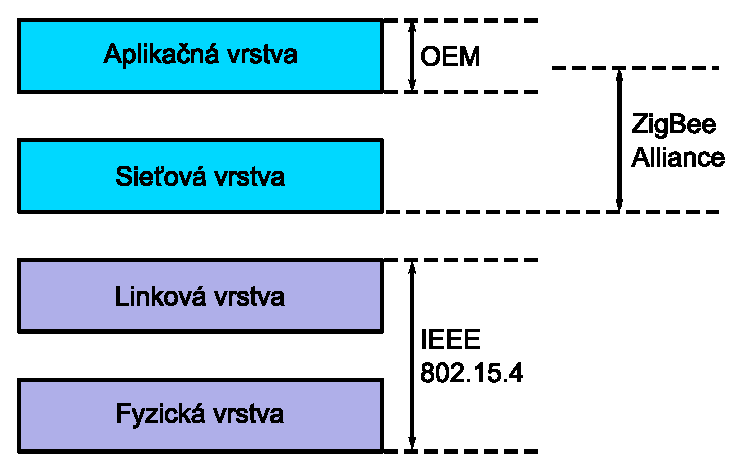
\includegraphics[width=140mm]{figures/zigbee_ieee}
\caption{Vzťah medzi ZigBee Alliance a IEEE 802.15.4}
\label{fig:zigbee_ieee}
\end{center}
\end{figure}
\indent Svojou charakteristikou sú siete ZigBee vhodné pre aplikácie nevyžadujúce vysoké nároky na datovú priepustnosť, uspokoja sa s bezdrôtovým spojením krátkeho dosahu, ale hlavne pre ktoré je kritická nízka energetická náročnosť. Tieto špecifiká posúvajú sie\-te ZigBee ako vhodného kandidáta pre bezdrôtové riadenie osvetlenia, termoreguláciu, bezpečnostné prvky v inteligentných domácnostiach, pre komunikáciu hlásičov požiaru v budovách, alebo aj v medicíne pre rýchle predávanie správ o stave pacienta do definovaného zberného bodu. V priemysle by zase táto technológia našla využitie napríklad v monitorovaní podmienok, v akých sa tovar nachádza v sklade (teplota, vlhkosť, vibrácie), alebo napríklad pri kontrole procesov v čističke odpadových vôd. Keďže sieť má vlastnosť samokonfigurácie, jej inštalácia aj vo väčších mierkach je otázkou zopár hodín.\\
\subsection{Architektúra ZigBee}
\indent\indent Architektúra siete ZigBee sa skladá zo štyroch základných vrstiev, ako zobrazuje aj obr.~\ref{fig:zigbee_ieee}. Tieto vrstvy medzi sebou komunikujú predávaním správ cez tzv. body prístupu služby (SAP - Service Access Point). SAP je v princípe miesto, v ktorom jedna v vrstiev môže požadovať služby druhej vrstvy. štruktúra architektúry spolu s vyznačenými SAP bodmi je vyobrazená na obrázku~\ref{fig:architecture_zigbee}. Na ňom môžme rozlišovať dva typy SAP bodov medzi jednotlivými vrstvami. Jeden typ predstavujú body, cez ktoré sú spracovávané užitočné dáta aplikácii (napr. MCPS-SAP, alebo PD-SAP) a druhý typ SAP bodov sa zaoberá manažmentom siete, ako napr. konfigurácia beacon rámcov, prípadne nastavovanie, alebo čítanie hodnôt atribútov (napr. MLME-SAP, PLME-SAP body).\\
\begin{figure}[htbp]
\begin{center}
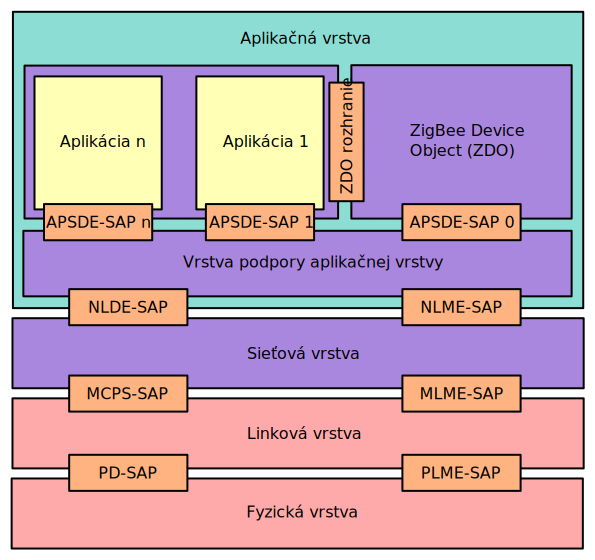
\includegraphics[width=140mm]{figures/architecture_zigbee}
\caption{Znázornenie vrstvovej architektúry siete ZigBee}
\label{fig:architecture_zigbee}
\end{center}
\end{figure}
\subsection{Sieťová vrstva}
\indent\indent Požiadavky na sieťovú vrstvu sú zabezpečovanie správneho fungovania linkovej vrstvy a poskytovania vhodných služieb vyššie postavenej aplikačnej vrstve. Podľa konceptu, sieťová vrstva obsahuje dve entity, ktorých služby sú využívané aplikačnou vrstvou. Tie\-to entity sú datová (NLDE - NWK Layer Data Entity) a manažement entita (NLME - NWK Layer Management Entity). Ku každej sa pristupuje cez príslušný bod SAP - NLDE-SAP, alebo NLME-SAP. Zmysel rozdelenia sieťovej vrstvy na tieto dve časti je v~tom, že NLME využíva NLDE pre vykonávanie potrebných úloh, ktoré majú charakter riadenia a kontroly na danej úrovni a takisto zabezpečuje prístup k sieťovej informačnej databázy (NIB - Network Information Base).\\
\subsection{Aplikačná vrstva}
\indent\indent Ako je ukázané na obrázku~\ref{fig:architecture_zigbee}, aplikačná vrstva sa skladá zo ZigBee Device Object objektu, z aplikačných objektov (definovaných výrobcom zariadenia, alebo aplikácie) a~z~podpornej vrstvy APS.\\
\subsubsection{Podporná vrstva aplikačnej vrstve}
\indent\indent Uvedená vrstva je v špecifikácii označovaná ako APS (Application Support Sub\-layer). Úlohy, ktoré jej prináležia si delia dve entity: datová (APSDE) a manažment (APSME). Datová ma na starosť sprístupnenie služieb pre aplikačné vrstvy v danej sieti a management entita zabezpečuje cez príslušný SAP bod funkcie bezpečnosti prenosu, prípadne prístup k informačnej báze danej podvrstvy. S podobným rozdelením sa budeme stretávať aj pri ostatných vrstvách protokolu.\\
\subsubsection{Objekty typu ZigBee Device Objects}
\indent\indent ZigBee Device Objects objekty (ZDO) hrajú dôležitú úlohu v protokole ZigBee. Pri štarte siete inicializujú sieťovú vrstvu a vrstvu APS. Na základe požiadavkov aplikácii dávajú impulz k procesom, ktoré realizujú vytváranie PAN, asociáciu do už existujúcej siete PAN, prípadne majú na starosť správu sieťovej vrstvy. Ako už bolo spomenuté v~\cite{halas03} ZDO môžme nazvať komunikačným bodom aplikačnej vrstvy. ZDO poskytuje funkcie pre všetky aplikácie bežiace na ZigBee zariadení vrátane skenovania siete (device and service discovery), vytvorenia spojení medzi objektami v sieti (binding) a správy šifrovacích kľúčov (security management). Vo výslednej simulácii je jediná z jej úloh inicializácia daného zariadenia spolu s nastavením základných parametrov pre spojenie. Na aplikačnej vrstve sú uvažované tzv. endpoints. Zariadenie môže mať nadefinovaných max. 240 endpoints a každému z nich zodpovedá jeden aplikačný profil. Pre ilustráciu môžme uviesť, že cez jeden endpoint je realizovaná komunikácia s cieľom zapnúť svetlo a cez iný endpoint môže aplikácia informovať iný ZigBee prvok o teplote prostredia zmeranej teplotným čidlom.\\
\subsection{Väzba na IEEE 802.15.4}
\indent\indent V špecifikácii k IEEE 802.15.4 sú uvedené aj doplnkové podvrstvy k základnéj vrstvovej štruktúre. Na mysli máme podvrstvy označované ako SSCS (Sublayer-Specific Convergence Layer) a LLC (Logical Link Control) vrstvy. Ich polohu znázorňuje obrázok~\ref{fig:architecture_sublayers}. Konvergenčná SSCS vrstva slúži k predávaniu informácii medzi sieťovou a~linkovou vrstvou. Následne má schopnosť informovať nadradené vrstvy o tom, v akom stave sa nachádza posielanie dát ostatným členom siete. Funkciou podvrstvy IEEE 802.2 LLC  je kontrola a zaistenie integrity dátových prenosov. LLC vrstva poskytuje cez body prístupu (SAP) služby linkovej vrstvy pre sieťovú vrstvu.\\
\begin{figure}[htbp]
\begin{center}
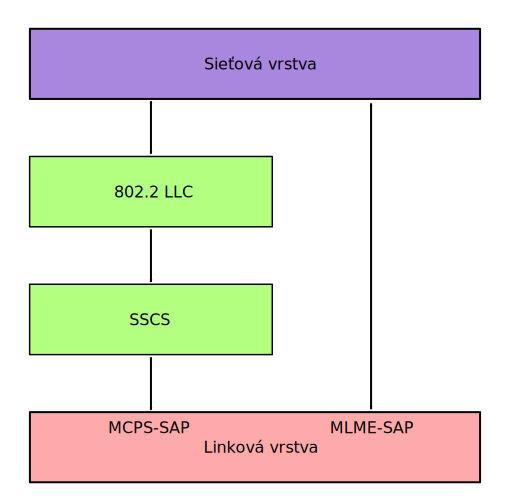
\includegraphics[width=120mm]{figures/architecture_sublayers}
\caption{Použitie doplňujúcich vrstiev v komunikácii medzi linkovou a sieťovou vrstvou}
\label{fig:architecture_sublayers}
\end{center}
\end{figure}

\cleardoublepage\chapter{Varianty simulačného modelu}

\indent\indent Vo svete okolo nástroja OMNeT++ sa za dobu od napísania našej predchádzajúcej práce venovanej simuláciám senzorových sietí udiali viaceré zmeny, ktoré nevyhnutne zasahovali aj do prípravy návrhu nášho simulačného modelu a museli byť zohľadnené. Zo všetkých týchto zmien je to posun dopredu, žiadna z nich sa neprejavila negatívne na našej práci.\\
\indent Simuačný nástroj OMNeT++ sa vyvinul do verzie 4.0, v ktorej najvýraznejšie úpravy sa dotkli jazyka NED (Network Definition Language) a datového typu premennej simulačného času \textit{SimTime}, ktorá teraz pracuje s vyšším rozlíšením. Ostatné úpravy sa veľmi nedotkli simulačného jadra, ako napríklad sú vyššia rýchlosť simulácii vo \textit{Fast} a \textit{Express} móde pri zapnutom GUI, alebo pre fanušíkov vývojárskych IDE zahrnutie IDE Eclipse upraveného pre potreby OMNeT++ modelov (podpora NED, a pod.).\\
\indent Okrem zmien vykonaných na samotnom simulačnom nástroji sa pokrok udial aj na scéne rozšírení do OMNeT++ a objavili sa okrem novšej verzie už široko používaného rozšírenia pre bezdrôtové siete Mobility Framework (v 2.0) aj nové rozšírenia pre senzorové siete: PAWiS a MiXiM.\\

\section{Rozšírenia pre simuláciu WSN sietí}

\subsection{PAWiS}
\indent\indent Celým menom PAWiS Simulation Framework~\cite{pawis_homepage} je rozšírenie cielené na simuláciu sietí typu WSN (Wireless Sensor Networks). Z toho dôvodu je značný dôraz kladený na správnu simuláciu správy napájania. Každá simulácia zahŕňa aj objekt \ttfamily Air\rmfamily, ktorý je obdobou modulu \ttfamily Channel Control \rmfamily z Mobility Framework. Modul \ttfamily Air \rmfamily realizuje výpočty spojené s útlmom signálu, ktorý je naviazaný na pohyb prvkov, teplotu prostredia, vibrácie zariadení, prípadne identifikuje útlm spôsobený prekážkami v priamej viditeľnosti medzi uzlami. Z praktického hľadiska funguje ako switch, do ktorého sa pripájajú všetky prvky a on následne preposiela rámce doplnené o vypočítaný útlm.\\
\indent Daný framework v podstate oproti zaužívanému Mobility Framework neponúka pre nás nič zaujímavé a nevideli sme žiadne benefity, ktoré by sme mohli využiť prechodom z MF na PAWiS. Jediná zaujímavosť v rozšírení PAWiS je uvedená správa napájania, ale tú, aj keď v jednoduchšej forme v podstate zvláda Mobility Framework doplnený o zásuvný modul Battery plugin~\cite{forster_homepage}.\\

\subsection{MiXiM}
\indent\indent Druhým novým produktom vo svete bezdrôtových simulácii je MiXiM. Tomuto nástroju sa povenujeme trochu hlbšie, pretože ponúka komplexnejší pohľad na simuláciu bezdrôtových sietí všeobecne. Projekt MiXiM spája v sebe vlastnosti viacerých rozšírení (okrem iného aj MF) a posúva simulačné možnosti o veľký krok ďalej.\\

\subsubsection{Vlastnosti}
\indent\indent Nástroj ponúka solídny základ pre modely a implementácie simulácii bezdrôtových sietí, vrátane modelov pre mobilné prostredia, propagáciu rádiových vĺn, podporu vo fyzickej vrstve pre modulácie a kódovania a takisto rozsiahlu knižnicu MAC protokolov a rôznych algoritmov. S čím prichádza MiXiM ako novinkou je práca s piatimi rozmermi, kde tri sú priestorové, jeden časový a piaty je frekvenčný. Vďaka tomu môžme skúmať vzájomné rušiace vplyvy rôznych kódovaní. V súvisloti so ZigBee sa vytvára vďaka nástroju MiXiM priestor pre povedzme pozorovanie vzájomného rušenia sa s nastupujúcim štandardom IEEE 802.11n (multifrekvenčný - OFDM, viacero antén - MIMO, variabliný bitrate pre hlavičku a telo správy, FEC). Modulárny dizajn pomáha pristupovať priamo aj ku komplexným situáciam a dovoľuje ľahko integrovať nové modely a implementácie protokolov. Prístup realizovaný simulátorom MiXiM je pekne popísaný v dokumente The MiXiM Vision~\cite{miximvision08}.\\

\subsubsection{Štruktúra}
\indent\indent Vlastnosti prostredia sú zahrnuté v module \ttfamily World\rmfamily . Modul \ttfamily World \rmfamily dokáže pracovať s 2-rozmerným aj 3-rozmerným priestorom (\ttfamily Playground\rmfamily). Ďalej MiXiM používa objekty, ktorými modeluje situáciu v prostredí, rôzne prekážky a podobne. Môžu to byť objekty charakteru budovy (\ttfamily ObjectHouse\rmfamily), alebo steny (\ttfamily ObjectWall\rmfamily). Tieto objekty nielen spôsobujú zmeny v šírení signálu, ale tiež kladú fyzické obmedzenia v mobilite prvkov. Správu takýchto objektov má na starosti modul nazývaný \ttfamily ObjectManager\rmfamily. Úlohu modulu \ttfamily ChannelControl \rmfamily z Mobility Framework prebral modul \ttfamily ConnectionManager\rmfamily. On dynamicky vytvára spojenia medzi uzlami tak, aby sa zbytočne nestrácal výpočtový výkon na simulovanie spojení, ktoré majú takmer nulovú váhu nielen čo sa týka kvality prenosu správ, ale aj z pohľadu príspevku k rušeniu na jednotlivých prijímačoch. Modul \ttfamily ConnectionManager \rmfamily sa vždy zaoberá výpočtom okolo jedného konrétneho typu vlnenia. To znamená, že pre spoločnú simuláciu dvoch rôznych sietí v pásme ISM 2.4~GHz a GSM 900~MHz budeme mať v simulácii 2 moduly typu \ttfamily ConnectionManager\rmfamily.\\ 
\indent Čo sa týka samotných uzlov, aj tu je vidieť, že ľudia, ktorí stoja za projektom MiXiM majú na svedomí aj projekt Mobility Framework. Štruktúra jednotlivých modulov v komunikačných uzloch je veľmi podobná tej z Mobility Framework (bližšie o nej v~\cite{halas03}). Sprostredkovanie prenosu informácii medzi jednotlivými modulmi už sa nedeje cez modul \ttfamily Blackboard\rmfamily, ale cez modul \ttfamily Utility\rmfamily. Ich funkcie sú totožné. Ďalej pribudol modul pre sledovanie spotreby a predikciu výdrže energie \ttfamily Battery \rmfamily a modul pracujúci so smerovacími mechanizmami \ttfamily Arp\rmfamily.\\
\indent Hlavná logika frameworku je ukrytá v moduloch a rozhraniach pre posielanie správ, ich transformácie do signálovej podoby a následné spracovanie prijatého signálu aj s informáciami o útlme a pod.

\paragraph{Signal}
\indent V simulácii signálu vstupuje u vysielacieho prvku do modelu faktor antény, prenosová rýchlosť, vysielací výkon a frekvencia (komunikačný kanál). Na prijímacej strane je výsledok ovplyvnený útlmom na prenosovom médiu, prijímacou anténou a aj útlmom spôsobeným prekážkami v linii priamej viditeľnosti, pretože, ako sme už spomenuli, práca s takýmito objektami je v istej podobe zvládnutá v simluačnom frameworku.

\paragraph{AnalogueModel}
\indent Miesto, v ktorom sú počítané uvedené faktory prijímaného signálu (útlmy, zisk antén).

\paragraph{Decider}
\indent Modul \ttfamily Decider \rmfamily rozhoduje o výslednom prijatí, alebo zahodení rámca, na základe rušenia a šumu. Aplikuje algoritmy FEC a tiež informuje nadradené vrstvy o stave prenosového média (busy/idle). Táto vrstva je miesto prechodu z analógového pohľadu na model na digitálny.

\paragraph{Radio}
\indent Bod, v ktorom sú prepínané stavy rádia (RX, TX, IDLE, SLEEP). Tieto stavy sú riadené vyššími vrstvami. Prípadne modul \ttfamily Radio \rmfamily môže obsahovať premenné, ktoré definujú rýchlosť prechodu medzi stavmi (napr. RX-to-TX time).

\paragraph{ChannelInfo}
\indent Pracuje s rámcami a komunikuje s vrstvou \ttfamily BasePhyLayer \rmfamily aby mohol do rámcov doplniť údaje doplňujúce dáta vyžadované modulom \ttfamily Decider\rmfamily. Dopĺňa rámce vypočítanými hodnotami premenných RSSI (Received Signal Strength Indication) a SINR (Signal to Interference plus Noise Ratio).

\paragraph{BasePhyLayer}
\indent Je čisto OMNeT++ modul. Komunikuje s vyššími vrstvami cez správy, ktorých obsach je popísaný výhradne NED jazykom.\\ \\
\indent Podrobné vzťahy sú schématicky vyobrazené na obr.~\ref{fig:architecture_mixim}.\\


\begin{figure}[htbp]
\begin{center}
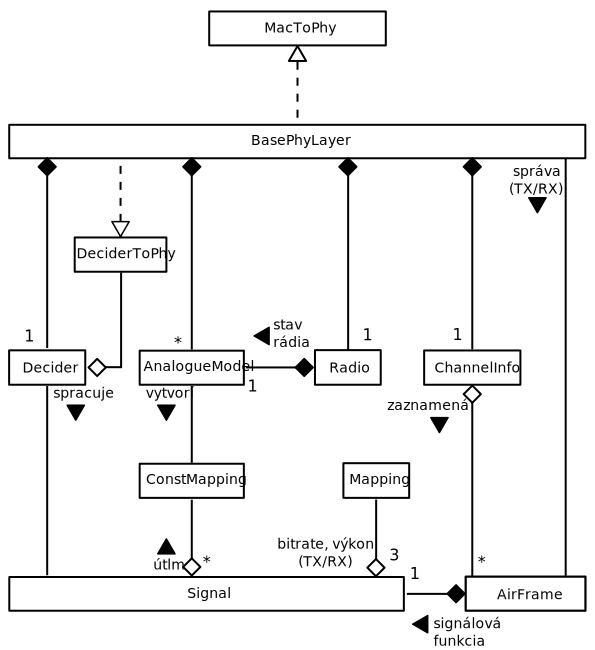
\includegraphics[width=140mm]{figures/architecture_mixim}
\caption{Práca so signálovou časťou simulácie vo frameworku MiXiM}
\label{fig:architecture_mixim}
\end{center}
\end{figure}

\subsection{Mobility Framework}
\indent\indent Mobility Framework~\cite{mf_homepage} je overený framework pre simulovanie bezdrôtových sietí postavený ako modul do simulátora OMNeT++. Medzi jeho nesporné výhody patrí jednoduchosť, prehľadnosť a rýchlosť behu simulácii. Nakoľko vývoj rozšírenia MiXiM sa zatiaľ nedostal do použiteľného stavu, ako najvýhodnejšie sa momentálne javí zostať pri frameworku MF. Ten sa medzičasom dočkal vývojovej verzie 2.0, v ktorej zostal vývoj zakonzervovaný, adaptovaný na verziu 4.0 nástroja OMNeT++ a už sa len odlaďujú chyby. Všetka vývojová snaha sa vkladá do nástroja MiXiM, ktorý je označovaný aj ako nepriamy nástupca MF.\\

\subsubsection{Architektúra}
\indent\indent V nástroji Mobility Framework sú použité isté zaujínavé riešenia, ktoré je vhodné si popísať a vďaka nim môžme potom lepšie pochopiť štruktúru návrhu simulačného modelu. K správe jednotlivých spojení sa pristupuje centrálne, pretože je potrebné poznať polohu všetkých komunikujúcich prvkov. Všetky spojenia sú vytvárané modulom \ttfamily ChannelControl \rmfamily dynamicky. Mobilita prvkov je spracovávaná individuálne, pretože každé so zariadení sa pohybuje nezávisle na ostatných a jediné, čo je potrebné, je oznámiť aktuálnu polohu modulu \ttfamily ChannelControl\rmfamily. Tento modul teda komunikuje s mobility modulmi, ktoré sú súčasťou každého jednotlivého prvku. Na obrázku je zobrazený princíp komunikácie medzi týmito modulmi. Dá sa povedať, že modul \ttfamily ChannelControl \rmfamily je jadrom celej mobility architektúry, pretože spojenia nielen vytvára, ale aj ruší v závislosti na vzdialenosti.\\

\paragraph{ChannelControl}
\indent Modul \ttfamily ChannelControl \rmfamily vytvára komunikačné kanály medzi prvkami, ktorých vzdialenosť nepresahuje určité medze a ruší ich tam, kde je kritická hodnota vzdialenosti presiahnutá. Každý kanál následne vyžaduje pár jednosmerných brán (\ttfamily gates\rmfamily) na oboch koncoch pre zabezpečenie obojsmernej komunikácie medzi prvkami. S uvedením OMNeT++ v4.0 boli síce predstavené v jazyku NED aj obojsmerné brány (typu \ttfamily inout\rmfamily), ale tie sa tiež len preložia pri kompiláci na 2 jednosmerné brány. Mobilita teda vyýaduje dynamicky sa meniaci počet brán. Vrámci efektívneho prístupu k správy pamäte sú brány nielen požadované, ale aj vytvárané dynamicky. Negatívum tohoto prístupu sa prejavuje pri zmene veľkosti vektora obsahujúceho zoznam brán, pretože každá zmena jeho veľkosti znamená nutnosť opakovaného napojenia všetkých brán, ktoré obsahuje, čo sa rovná počtu všetkých brán v simulácii. Následne bol nájdený kompromis v tom, že brány sa vytvárajú a rušia nie po štyroch (najmenšie kvantum, týka sa jedného spojenia), ale po väčších zhlukoch.\\
\indent Udržovanie stavu o spojeniach je výpočtovo drahá úloha so zložitosťou $O(n^2)$. Aj v tejto oblasti MF pristupuje k problému so zjednodušením. \ttfamily ChannelControl \rmfamily udržuje teda informácie o spojeniach len tých, ktoré sú v rozumnom komuniačnom rozsahu. Po inicializácii \ttfamily ChannelControl \rmfamily rozhodne o interferenčnej vzdialenosti pri ktorej ešte uzly siete stále môžu vzájomne rušiť komunikáciu. \ttfamily ChannelControl \rmfamily túto vzdialenosť vie odhadnúť na základe hraničnej threshold hodnoty SNR (Signal-to-Noise Ratio). Celá sieť je rozdelená na kvadranty, ktorých dĺžka strany predstavuje práve spomínanú interferenčnú vzdialenosť. To potom znamená, že uzol v danej zóne môže interferovať len s uzlom nachádzajúcim sa v tej istej, alebo susednej zóne. Pohľad na situáciu, v ktorej sa automaticky nepočíta so spojeniami medzi uzlami o ktorých vieme, že sú od seba vzdialený na väčšiu dĺžku, ako je interferenčná vzdialenosť je na obr.~\ref{fig:channelcontrol_areas}. Pre každú z týchto interferenčných zón je udržovaný zoznam obsiahnutých uzlov, ktoré sa v nej nachádzajú. V konečnom dôsledku \ttfamily ChannelControl \rmfamily prepočítava len spojenia medzi uzlami z vybraných zoznamov a nie medzi všetkými uzlami v sieti. Samozrejme, zložitosť predstaveného algoritimu je silne závislá na hustote uzlov.\\

\begin{figure}[htbp]
\begin{center}
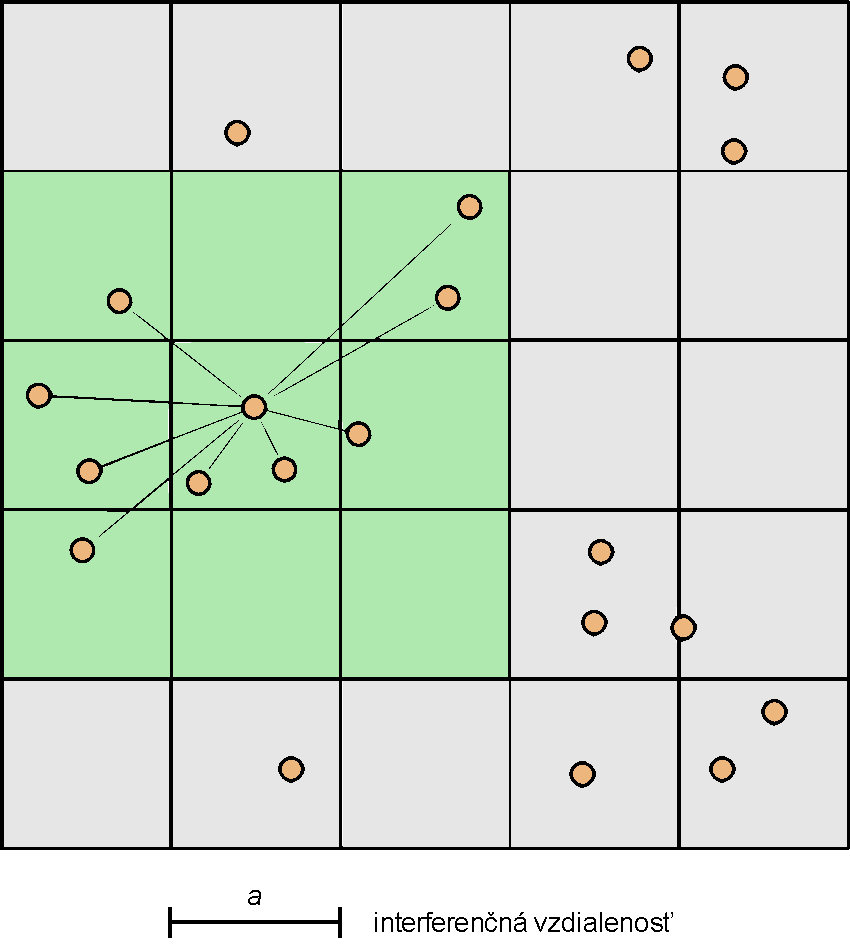
\includegraphics[width=120mm]{figures/channelcontrol_areas}
\caption{Ignorovanie spojení medzi uzlami z kvadrantov, ktorých vzdialenosť presahuje hodnotu interferenčnej vzdialenosti}
\label{fig:channelcontrol_areas}
\end{center}
\end{figure}

\paragraph{Mobility}
\indent Je prirodzené, že každý uzol bude zodpovedný za svoj pohyb po priestore. Teda mobilita zariadení je realizovaná distribuovane v každom uzle. Je riadená modulom \ttfamily Mobility\rmfamily, ktorý je obsiahnutý v štruktúre každého uzla. Aj toho statického, pretože \ttfamily Mobility \rmfamily pridáva k vysielanému rámcu dáta pre \ttfamily ChannelControl\rmfamily, vďaka ktorým je známa poloha prvku a môžu sa prepočítať ich vzájomné vzdialenosti medzi uzlami. Pre zníženie náročnosti je volaná priamo metóda na objekte \ttfamily ChannelControl\rmfamily. Ušetria sa tým prostriedky na správu ďalších brán, vytváranie nových správ a ich rušenie u príjemcu. Zásluhou modulu \ttfamily Mobility \rmfamily je aj aktualizovaný pohľad na simulačné pole pri zapnutom GUI počas simulácie. Smer komunikácie medzi \ttfamily ChannelControl \rmfamily a \ttfamily Mobility \rmfamily modulmi v rôznych uzloch je ilustrovaný na obr.~\ref{fig:topology_mobility}.\\

\begin{figure}[htbp]
\begin{center}
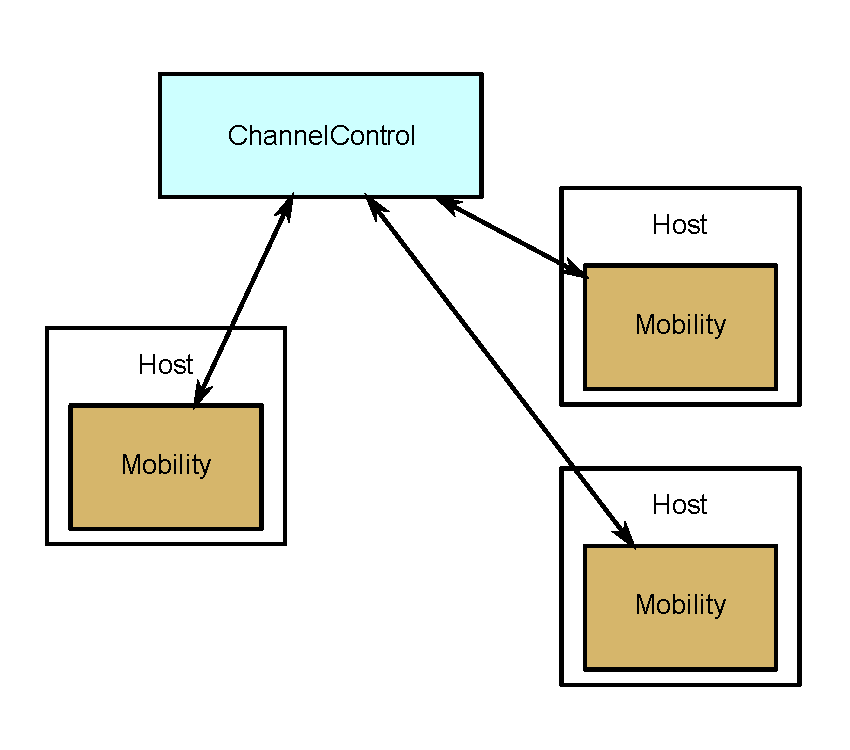
\includegraphics[width=120mm]{figures/topology_mobility}
\caption{Komunikácia medzi modulmi \ttfamily Mobility \rmfamily a \ttfamily ChannelControl\rmfamily}
\label{fig:topology_mobility}
\end{center}
\end{figure}

\paragraph{Blackboard}
\indent Koncept Blackboard sprostrekúva komunikáciu medzi typu od jedneho k mnohym (one-to-all). Je súčasťou každého hostu a vďaka nemu prebieha výmena informácii aj medzi tými vrsvtami, ktoré nemaju spoločný komunikačný kanál. Komunikácia potom prebieha spôsobom zverejňovania informácii (publish) na Blackboard a pripísaniu sa k odberu týchto informácii (subscribe). V konečnom dôsledku príjemca má možnosť zistiť, kto bol pôvodcom informácie. Moduly, ktoré sú prihlásené k odberu správ sú upozornené v prípade, že dáta, o ktoré mali záujem, boli sprístupnené alebo aktualizované. V ďalšom kroku ich potom môžu prečítať.\\
\indent Príklad efektívneho použitia tohoto modulu si môžme predstaviť pri bezdrôtovej komunikácii pomocou metódy CSMA-CA, kedy po odoslaní správy sa rádio môže prepnúť do stavu RX a túto informáciu zverejní na Blackboard. Vďaka tomu potom povedzme modul, ktorý simuluje energetické zdroje vie, že príkon rádia sa zmenil a zároveň o túto informáciu má záujem aj linková vrstva, ktorá vďaka nej vie, že správa bola odoslaná.\\

\paragraph{Decider}
\indent Modul decider spracováva informáciu vyslanú fyzickou vrstvou, pomocou použitej modulačnej schémy spočíta hodnoty BER (Bit Error Rate) a prípadne označí bity prijaté s chybou. Tento modul je špeciálne užitočný pri pracovaní s datovými tokmi s premenlivou priepustnosťou (rozdielny bitrate hlavičky a tela - IEEE 802.11) a tým, že je oddelený od ostatných zložiek fyzickej vrstvy umožňuje programátorovi ľahšie aplikovať zmenu použitej modulačnej schémy pri simulácii.\\

\section{Existujúce modely sietí ZigBee a IEEE 802.15.4}
\indent\indent Po ponúknutí vhodných simulačných nástrojov si viacero skupín vybralo práve protokol IEEE 802.15.4. Doôvody môžu byť rôzne - mobilita prvkov, bezdrôtová komunikácia, jednoduchá implementácia, prípadne analýza mechanizmu GTS. Z uvedených nástrojov vzťahujúcich sa k simulátoru OMNeT++ sú k dispozícii viaceré čiastočné implementácie protokolu IEEE 802.15.4. V krátkosti ich popíšeme na v tejto kapitole.\\

\paragraph{PAWiS (Institute of Computer Technology, Vienna University of Technology)}
\indent Simulátor PAWiS ponúka základ pre linkovú vrstvu ZigBee protokolu. Pri analýze zdrojového kódu tejto vrstvy sa ukázalo, že to nie je ani hrubý základ MAC vrstvy. V zjednodušenej podobe zvláda CSMA algoritmus. Spomedzi knižníc simulačného daného nástroja sa jedná o vedľajší produkt.

\paragraph{MiXiM}
\indent Aj v simulátore MiXiM je pripravená implementácia štandardu IEEE 802.15.4. Táto je totožná s tou z Mobility Framework, je z nej portovaná. Podrobnejšie si ju rozoberieme v nasledujúcom odstavci.

\paragraph{MF (Jérôme Rousselot)}
\indent V Mobility Framework vo verzii 2.0 preview 1 sa objavila v istej podobe naimplementovaná linková vrstva protokolu IEEE 802.15.4. Táto implementácia je čistou implementáciou algoritmu CSMA-CA. Veci ako podpora pre \textit{SLEEP} mód rádia, pre GTS sloty, osirotenie, alebo beacon rámce v nej nie je obsiahnutá. Podoby uvedeného modelu sú dve. Predstavujú implementácie kariet Texas Instruments CC 2420 802.15.4 a Texas Instruments CC 1100 802.15.4, a to pre frekvenčné pásma 868~MHz a 2.4~GHz. Podľa toho sú následne nastavené okrem hodnoty frekvencie nosnej aj veľkosti hlavičiek rámcov, dĺžka SFD (Starting Frame Delimiter), hodnoty viacerých časovačov (napr. ACK timeout).

\subparagraph{MF (Autor)}
\indent Naša predchádzajúca práca venovaná simulácii WSN sietí~\cite{halas03} bola doplnená o jednoduchú implementáciu fyzickej, linkovej a sieťovej vrstvy protokolov ZigBee a IEEE 802.15.4. Táto implementácia obsiahla procedúry pre vytvorenie siete PAN koordinátorom, správu asociácii a vysielanie beacon rámcov.\\
\indent Tým, že som sa podielal na príprave tohoto modelu, sme mali pôvodne zámer ho rozšíriť a doplniť chýbajúce procedúry. Okrem toho  sa uvolnili nové verzie štandardov ZigBee a aj IEEE 802.15.4, čo sme tiež chceli reflektovať v našom novom modeli. Vtedy sa ale ukázal prvý nedostatok nášho prvého produktu. Nízka modularita. Úprava na štandard IEEE 802.15.4b-2006 by si vyžiadala relatívne veľké zásahy. Ďalšie negatívum, bolo zlúčenie modelu fyzickej vrstvy ako je definovaná v dokumente a fyzickej vrstvy ako ju poníma Mobility Framework. Toto pri našej práci nebolo silnou prekážkou, no v prípade, že sa nájde záujemca o použitie nášho modelu vo frameworku MiXiM, ktorý má tendenciu stať sa náhradou za MF, spraví mu naša implementácia fyzickej vrstvy zopár starostí. A ako jednu z posledných vecí, kde by sme zmenili prístup je komunikácia medzi vrstvami, kedy sme preposielanie riadiacich inštrukcii riešili cez modul \ttfamily Blackboard\rmfamily. Teraz sa budeme snažiť výhradne o preposielanie správ. \ttfamily Blackboard \rmfamily bude slúžiť na prenos riadiacich a stavových informácii medzi časťou fyzickej vrstvy ako je k nej pristupované z pohľadu MF a ako časťou fyzickej vrstvy, ako je popísaná v štandarde.



\cleardoublepage\chapter{Popis simulačného modelu}
\indent\indent Simulátor MiXiM sa v čase písania tejto práce vyvíjal relatívne dynamicky. Avšak v~podobe, v ktorej sa nachádzal, ešte neumožňoval plnohodnotnú prípravu modelu a dynamika jeho vývoja bola skôr na príťaž ako na osoh. To bol hlavný motív, prečo zostať pri Mobility Framework rozšírení. Našou snahou teda bolo pripraviť taký modul, ktorý sa bude dať vo vhodnej chvíli ľahko transformovať do podoby vhodnej pre simulačný framework MiXiM.\\
\indent Toto sa podarilo tak, že fyzickú vrstvu sme rozdelili na 2 časti. Jedna je napísaná spôsobom, aby vedela spracovávať formáty správ definované IEEE 802.15.4b-2006 štandardom, aby sekvencie udalostí, ktoré v nej prebiehajú, boli zodpovedajúce štandardu. Táto vrstva ale nekomunikuje priamo s modulom \ttfamily ChannelControl\rmfamily, ale predá správy druhej časti fyzickej vrstvy, a tá už je implementovaná v podobe, ktorá silno závisí na konkrétnom použitom rozšírení modulu OMNeT++. Medzi týmito dvoma základnými časťami komunikácia prebieha vo forme oznamov cez modul \ttfamily Blackboard \rmfamily a aj cez predávanie správ pomocou komunikačných brán. Komunikácia pomocou definovaných brán medzi uvedenými úrovňami fyzickej vrstvy sa deje výhradne za účelom preposielania správ na médium, alebo príjmu správ z prijímača.\\
\indent Aby sa zabezpečilo bezproblémové nasadenie mobility architektúry a prenos IP paketov sieťou IEEE 802.15.4, implementovali sme robustný model fyzickej a linkovej vrstvy. V zásade sme dodržali členenia na vrstvy tak, ako ho prezentuje štandard. To znamená implementovali model fyzickej (PHY) a linkovej (MAC) vrstvy z dokumentu IEEE 802.15.4~\cite{ieee06} a sieťová vrstva (NET) a aplikačná (APP) je pripravená podľa dokumentu Zig\-Bee Specification~\cite{zigbee08}. Medzi týmito vrstvami sú preposielané správy, ktoré sa v~podstate delia do dvoch základných skupín:\\
\begin{itemize}
 \item správy, obsahujúce užitočné dáta aplikácii
 \item správy, ktoré majú riadiaci charakter
\end{itemize}
\indent\indent Charakter komunikácie medzi jednotlivými vrstvami a návrh rozdelenia PHY vrstvy je vyobrazený na obr.~\ref{fig:architecture_model}.\\
\begin{figure}[htbp]
\begin{center}
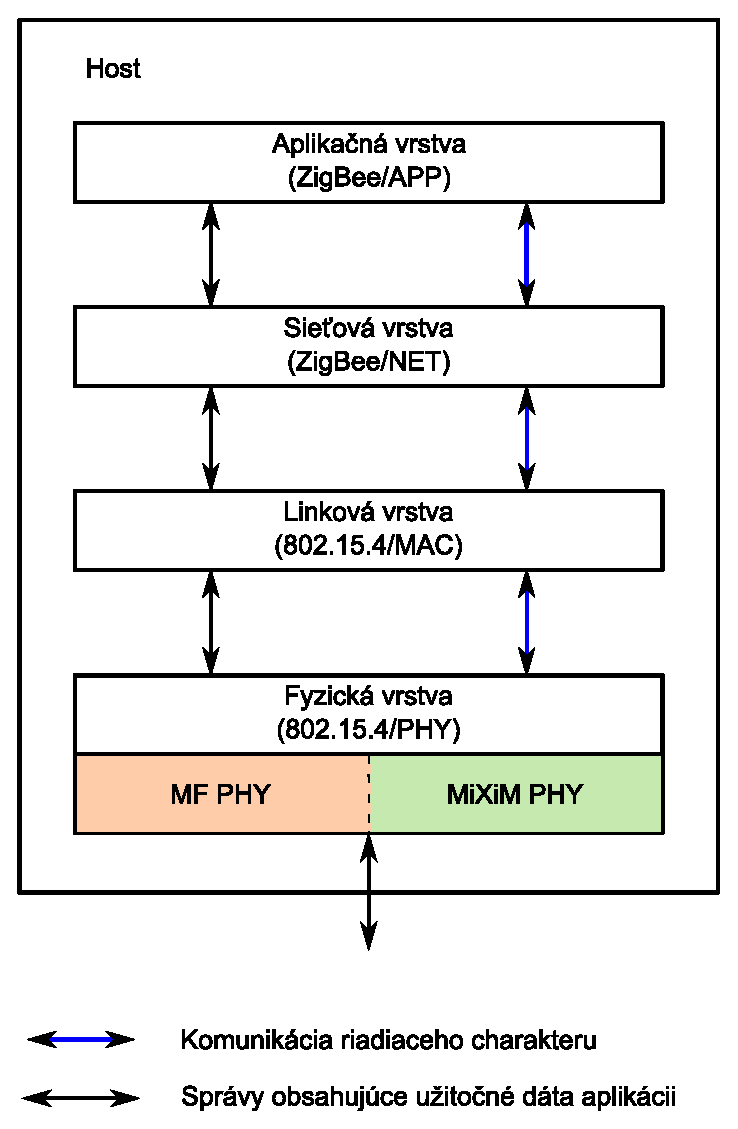
\includegraphics[width=120mm]{figures/architecture_model}
\caption{Základný pohľad na nami navrhovaný simulačný model}
\label{fig:architecture_model}
\end{center}
\end{figure}
\indent\indent Štruktúra jednotlivých vrstiev modelu sa ďalej člení na isté bloky, ktoré na každej z týchto vrstiev pracujú s presne definovanými správami. Jeden blok má na starosti spracovávanie riadiacich informácii, druhá časť vrstvy správy enkapsuluje pri postupe informácie v smere nadol v hierarchii vrstiev (dekapsuluje pri smere nahor). Oba tieto bloky samozrejme medzi sebou komunikujú. Ako tretí prvok v tejto štruktúre je databáza konfiguračných premenných, z ktorých časť má charakter konštánt a má teda dovolený len prístup na čítanie. K ostatným je povolený aj zápis, samozrejme len v~rámci medzí hodnôt, ktoré dovoľujú štandardy.\\
\indent Z ďalších vecí je zahrnutá podpora pre FFD a RFD zariadenia. Úloha uzlov je diverzifikovaná na úrovni aplikačnej vrstvy.\\

\section{Aplikačná vrstva - APP}
\indent\indent Čo sa týka aplikačnej vrstvy, mala by obsahovať vrstvu podpornú aplikačnej vrstvy (APSDE). Tú sme vynechali z dvoch dôvodov. Prvým a najdôležitejším, je ten, že nachádzame sa v oblasti, ktorej podoba silne závisí od výrobcov zariadení (OEM - Original Equipment Manufacturer) a konkrétnych účelov, pre ktoré bolo ZigBee zariadenie vyrobené. Druhým je, že pri získavaní dát o kvalite a rýchlosti algoritmov, ktoré najviac ovplyvňujú a charakterizujú siete ZigBee nemá aplikačná vrstva veľkú váhu. Aplikačná vrstva v nami danej podobe má úlohu spustiť procesy pre zmonitorovanie prostredia, pre zostavenie PAN siete. V ďalšom kroku povolí na nami definovaný interval (akceptuje sa aj nekonečne dlhý interval - hodnota premennej \textit{permitDuration} $0xFF$) FFD zariadeniam asociovať ďalšie prvky do siete.\\

\section{Sieťová vrstva - NET}
\indent\indent Sieťová vrstva je členená bloky (obr.~\ref{fig:topology_net}), každý z nich si plní svoje špecifické úlohy. Funkcie týchto blokov zodpovedajú ich popisu v ZigBee špecifikácii. Od sieťovej vrstvy sa požaduje poskytovanie funkcionality a zaistenie vhodných služieb pre správne fungovanie IEEE 802.15.4b-2006 linkovej vrstvy. K rozhraniu smerom k aplikačnej vrstve, ponúka koncept sieťovej vrstvy služby dvoch funkčných blokov. Tieto bloky sú označované ako datová (NLDE - Network Layer Data Entity) a riadiaca (NLME - Network Layer Management Entity).\\
\begin{figure}[htbp]
\begin{center}
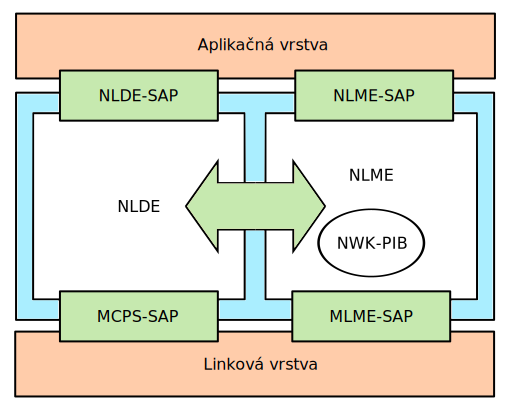
\includegraphics[width=120mm]{figures/topology_net}
\caption{Referenčný model sieťovej vrstvy}
\label{fig:topology_net}
\end{center}
\end{figure}
\subsection{Datová entita - NLDE}
\indent\indent Blok NLDE  (Network Layer Data Entity) poskytuje datové služby, ktoré dovolia aplikácii prenos im vlastných datových jednotiek (APDU - Application Protocol Data Unit) medzi viacerými zariadeniami na jednej PAN sieti. V princípe NLDE poskytuje služby:
\begin{itemize}
\item Vytváranie a spracovávanie datových jednotiek sieťovej vrstvy (NPDU - Network level PDU)
\item Smerovanie NPDU cieľovému zariadeniu v závislosti od topológie
\item Zaistenie autentizácie a utajenia prenosu, ak je vyžadované
\end{itemize}
\subsection{Riadiaca entita - NLME}
\indent\indent Riadiaca entita sieťovej vrstvy NLME (Network Layer Management Entity) podľa špecifikácie vykonáva tieto úlohy:
\begin{itemize}
\item Konfigurácia nových zariadení
\item Založenie novej siete
\item Pripájanie sa do existujúcich sietí (či už v rámci štartovacej sekvencie zariadenia, alebo po osirotení)
\item Prideľovanie 16-bitových adries podľa zabudovaného algoritmu
\item Udržovanie si zoznamu susediacich prvkov v dosahu rádia
\item Dáva k dispozícii viaceré smerovacie algoritmy v závislosti od charakteru vyžadovaného prenosu (unicast, multicast, broadcast)
\end{itemize}
\paragraph{Implementácia}
Implementácia sieťovej vrstvy počíta s rozdelením na 3 jednoduché moduly v jazyku NED. Tieto budú NLME, NLDE a NWK-PIB (Network layer Protocol Information Base). Moduly NLME a NLDE budú pripojené pomocou párov jednosmerných brán k~aplikačnej vrstve. Takisto sa počíta so zasielaním správ priamo medzi modulmi NLME a NLDE, preto aj v tomto mieste bude otvorená komunikačná cesta. Ako tretí bude jednoduchý modul NWK-PIB. Tento nebude pripojený k žiadnemu inému modulu komunikačnými bránami, ale bude obsahovať nadefinované verejne prístupné metódy (\texttt{public}) slúžiace na zapisovanie hodnôt atribútov a čítanie hodnôt atribútov a konštánt pre sieťovú vrstvu.\\
\indent Vrstva NLME tiež obsahuje datovú štruktúru reprezentujúcu mapu susediacich prvkov \texttt{std::map<unsigned long, NeighborTableEntry>}. Každý z týchto prvkov je identifikovaný 64-bitovým kľúčom - IEEE adresou. Záznam v tabuľke \texttt{NeighborTableEntry} obsahuje polia tak, ako sú pre tabuľku susedov definované v ZigBee špecifikácii.\\
\indent Ďalej si modul NLME uchováva aj informácie o PAN sietiach vo svojom okolí a v prípade FFD prvku tiež zaznamenáva počet asociovaných potomkov do siete a ich charakter (koncové zariadenie/smerovač) pre správne fungovanie distribuovaného mechanizmu prideľovania sieťových adries. Ak si zariadenie ukladá do \textit{neighborTable} záznam o smerovači, tak v tomto zázname je obsiahnutá aj informácia \textit{incomingBeaconTimestamp}, ktorá hovorí o relatívnej dobe prijatia beacon rámca od daného zariadenia. Hodnota je udaná v symboloch. Mimo to záznam v tabuľke, obsahuje ešte údaj v symboloch o~časovom odstupe beacon rámca vysielaného susediacim prvkov a prijímaného susediacim prvkom od jeho rodiča v topológii siete. Vďaka kombinácii týchto dvoch údajov si vie potom ďalší prvok účinne naplánovať vysielanie beacon rámcov tak, aby nespôsobovalo konflikty s inými beacon rámcami.\\
\indent Sieťová vrstva cez svoj modul NLME zapisuje do MAC-PIB (Medium Access Control layer Protocol Information Base) modulu linkovej vrstvy cez primitívu MLME-SET.request časť obsahu beacon rámcov označovanú ako \textit{macBeaconPayload}. Sú to informácie pre sieťové vrstvy susediacich prvkov, ktoré sú podávané cez implementovanú komunikačnú primitívu MLME-BEACON-NOTIFY.indication.\\
\indent K týmto trom základným blokom (NLDE, NLME, NWK-PIB) je pridaný blok \textit{Arp}. Idea tohoto riešenia je v separovaní smerovacieho algoritmu v extra module z dôvodu jeho prehľadnejšieho ladenia a ľahkosti v prípadnom experimentovaní s použitím iných smerovacích algoritmov.\\
\begin{figure}[htbp]
\begin{center}
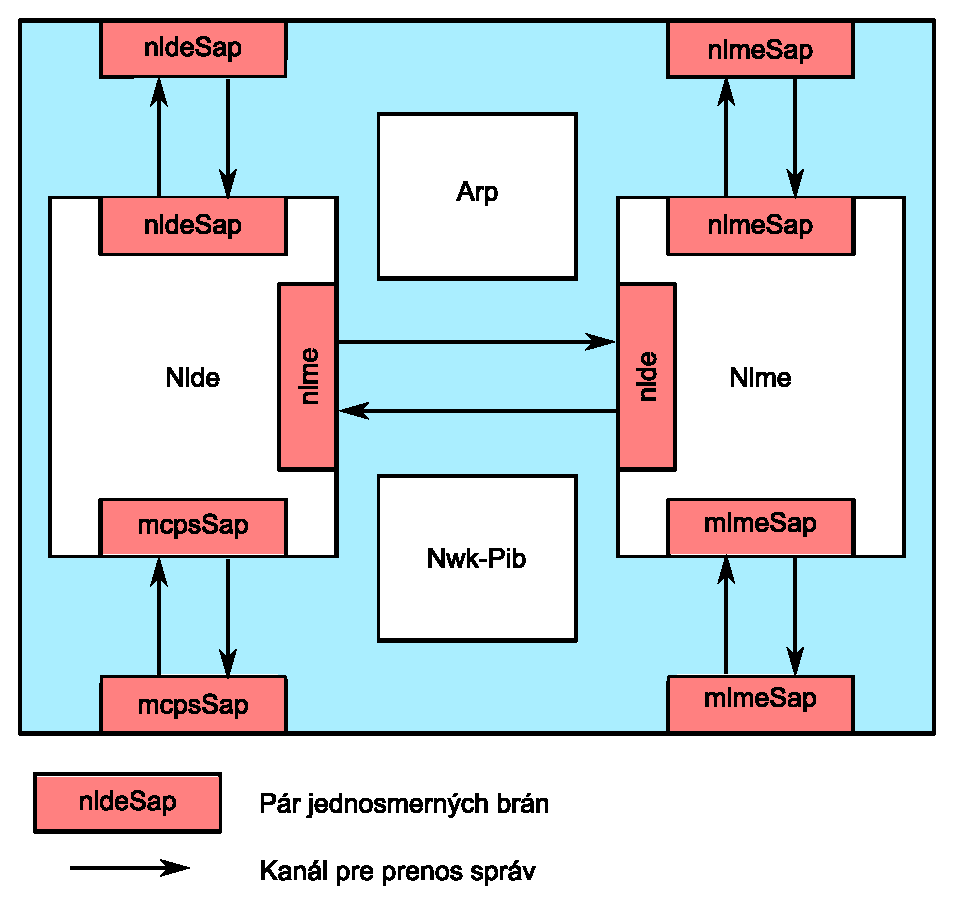
\includegraphics[width=120mm]{figures/architecture_net}
\caption{Podoba implementovaného modelu sieťovej vrstvy}
\label{fig:architecture_net}
\end{center}
\end{figure}

\section{Linková vrstva - MAC}
\indent\indent Úlohou linkovej vrstvy je riadiť prístup na prenosové médium a spracovávať informácie prijaté rádiom. V prípade linkovej vrstvy sú entity použité tiež dve - datová (MCPS - MAC Common Part Sublayer) a riadiaca (MLME - MAC Layer Management Entity). Okrem toho, že ponúkajú služby sieťovej vrstve cez príslušné body služby (SAP), existuje medzi nimi rozhranie, ktoré zabezpečuje riadiacej MLME entite využívať datové služby entity MCPS. Linková vrstva dokáže pracovať v 2 režimoch - beacon enabled a~non-beacon enabled móde. V prípade beacon-enabled módu prvok v roli smerovača v pravidelných intervaloch vysiela beacon rámec. Periodicita vysielania tohoto rámca je daná hodnotou premennej \textit{macBeaconOrder}. V prípade hodnoty $macBeaconOrder = 0x0F$ pracuje sieť v non-beacon enabled móde a beacon rámce sú zasielané len na vyžiadanie. V našom modeli sme sa vyhli implementácii tohoto módu, pretože podobné implementácie v simulátore OMNeT++ už existujú. Mimo to, úlohy linkovej vrstvy sú delené do dvoch skupín v závislosti od funkcionality, ktorá je od nich požadovaná:
\paragraph{FFD funkcionalita}
\begin{itemize}
\item Fungovanie v akejkoľvek topológii
\item Schopnosť fungovať v roli PAN koordinátor
\item Schopnosť komunikovať s akýmkoľvek IEEE 802.15.4 zariadením v PAN sieti
\item Implementovaná kompletná sada protokolu IEEE 802.15.4
\end{itemize}
\paragraph{RFD funkcionalita}
\begin{itemize}
\item Funkcia obmedzená na hviezdicovú topológiu, alebo rolu end-device v peer-to-peer móde
\item Nemožnosť vytvoriť sieť a stať sa PAN koordinátorom
\item Komunikácia len s FFD zariadením
\item Jednoduchá implementácia
\item Nízka spotreba energie
\end{itemize}
\begin{figure}[htbp]
\begin{center}
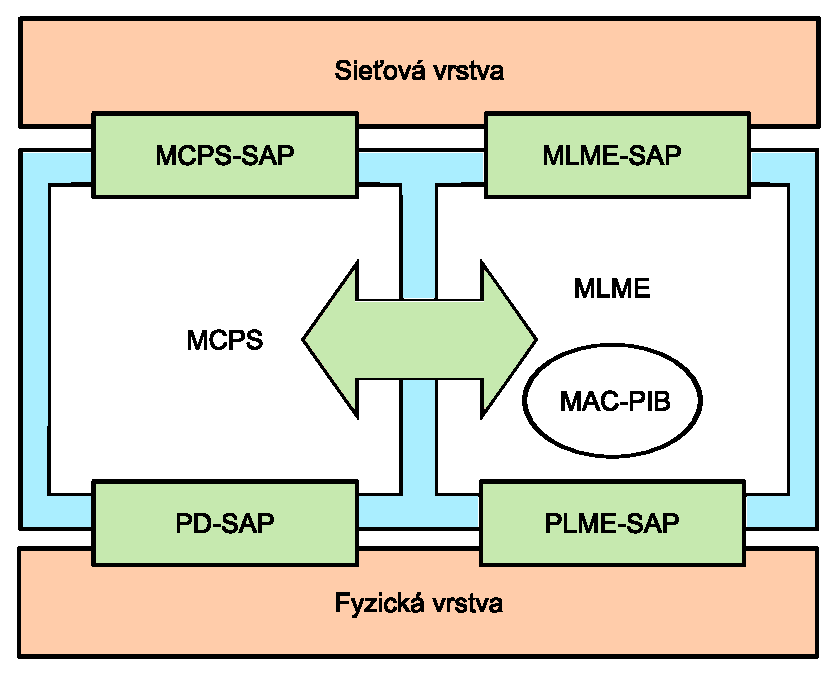
\includegraphics[width=120mm]{figures/topology_mac}
\caption{Referenčný model linkovej vrstvy}
\label{fig:topology_mac}
\end{center}
\end{figure}
\indent\indent Všetky zariadenia komunikujú na linkovej úrovni pomocou 64-bitových IEEE adries, alebo 16-bitových adries pridelených sieťovou vrstvou. Každá PAN sieť má pridelený svoj exkluzívny identifikátor. Tento identifikátor v kombinácii s cieľovou adresou definuje príjemcu komunikácie. Hodnota 16-bit sieťového identifikátora $0xFFFF$, alebo hodnota 16-bit PAN identifikátora $0xFFFF$ predstavuje broadcast adresu. Prijatý rámec, ktorý obsahuje takýto cieľový PAN identifikátor, alebo cieľovú sieťovú adresu nie je zahodený a je spracovaný linkovou vrstvou. Kontrola toho, či dané zariadenie je adresátom prijatého rámca, je vykonávaná vo vrstve MCPS.\\
\subsection{Datová entita - MCPS}
\indent\indent Modul MCPS slúži na prenos SPDU (SSCS Protocol Data Unit) medzi viacerými SSCS entitami.\\
\paragraph{Implementácia}
Datová entita MCPS využíva pre prenos rámcov fronty. Naša implementácia používa tieto fronty dve. Jednu pre prenos správ v perióde CAP pri beacon enabled móde alebo pre prenos riadiacich správ s vyššou prioritou v non-beacon enabled móde a druhú pre prenos správ v móde non-beacon enabled, ktoré majú nižšiu prioritu. Do týchto front sú rámce vkladané hneď po zapúzdrení (enkapsulácii). Teda vrstva MCPS sa stará aj o~enkapsuláciu. Niekedy nemá potrebné informácie k enkapsulácii rámca, ktorý je poslaný z~povedzme NLME vrstvy, vtedy NLME využije datovej štruktúry \texttt{nextEncapsulation} a~nastaví v nej príslušné hodnoty. To sa týka parametrov, ktoré nie sú obsiahnuté v správach generovaných NLME vrstvou, ale sú potrebné pre korektnú enkapsuláciu daného paketu (obr.~\ref{fig:frame_mac}). Simulačný model sa nezaoberá bezpečnosťou, preto je pole Auxiliary Security Header vždy dĺžky $0$.\\
\indent Modul MCPS posiela rámce potvrdení, ak sú vyžadované. Používa k tomu časovač \textit{ackTimer}. Modul MCPS ďalej dodržiava časové odstupy medzi datovými rámcami a~ACK rámcami. Sú to intervaly dané štandardom, ktoré dávajú zariadeniam čas na spracovani prijatých rámcov. Spôsob dodržovania týchto odstupov je vyobrazený na obr.~\ref{fig:interframe_spacing}.\\
\begin{figure}[htbp]
\begin{center}
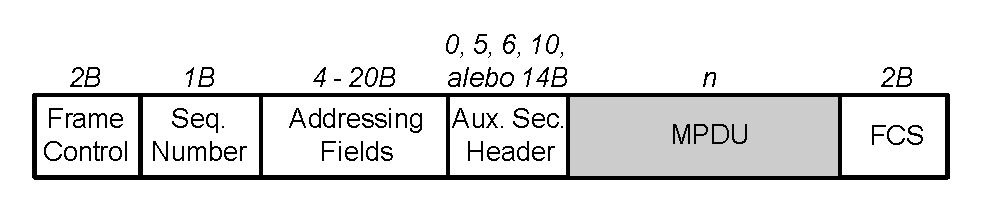
\includegraphics[width=140mm]{figures/frame_mac}
\caption{Spôsob enkapsulácie MPDU na linkovej vrstve}
\label{fig:frame_mac}
\end{center}
\end{figure}
\begin{figure}[htbp]
\begin{center}
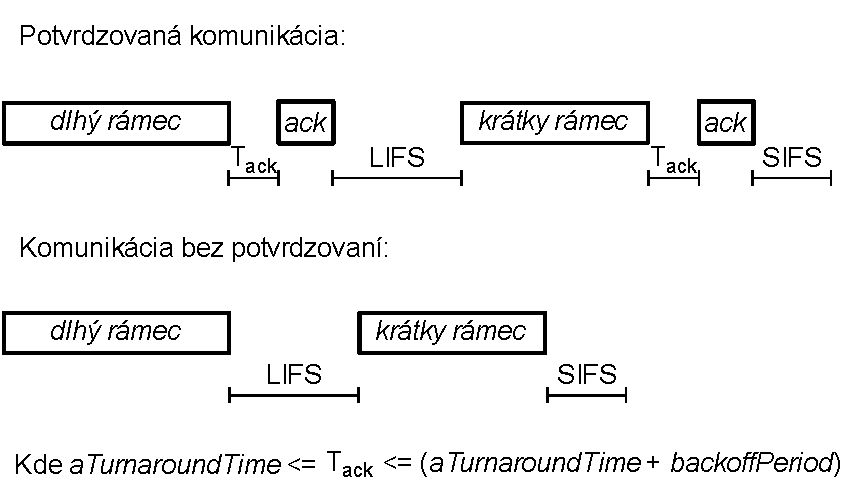
\includegraphics[width=120mm]{figures/interframe_spacing}
\caption{Minimálne časové odstupy medzi jednotlivými rámcami}
\label{fig:interframe_spacing}
\end{center}
\end{figure}
\subsection{Riadiaca entita - MLME}
\indent\indent MLME vrstva v časovom intervale označovanom ako CFP (viď obr.~\ref{fig:superframe}) realizuje prístup na médium cez tzv. CSMA-CA mechanizmus. CSMA mechanizmus znižuje pravdepodobnosť kolízie rámcov pri vysielaní viacerých rádii na spoločnom prenosovom médiu. Konkrétna aktivita CSMA mechanizmu sa nastavuje týmito parametrami:
\begin{itemize}
\item \textit{backoffExponent} (východzia hodnota: \textit{macMinBE})
\item \textit{numberOfBackoffs} (východzia hodnota: $0$)
\end{itemize}
\indent\indent CAP perióda je delená do 16 rovnako dlhých superframe slotov. Procedúra pre zistenie, či sa médium nachádza v stave \textit{idle} sa označuje ako Clear Channel Assessment (CCA) a vždy začína spolu so začiatkom nového superframe slotu. Prvý superframe slot je dedikovaný vysielaniu beacon rámca. Požiadavka na vysielanie rámca pomocou CSMA-CA mechanizmu začína po prvý krát vždy počas prvého superframe slotu. Keďže počas neho je vysielaný beacon rámec, CCA procedúra procedúra zistí, že kanál nie je voľný a začína tzv. backoff interval. Tento backoff interval hovorí o počte uplynutých superframe slotov pred ďalším pokusom o vyslanie rámca. Vypočíta sa ako náhodné číslo z intervalu $<0, 2^{backoffExponent})$. Po neúspešnom pokuse o vyslanie rámca sa zvýši hodnota \textit{backoffExponent} o jednotku a hodnota \textit{numberOfBackoffs} tiež o jednotku. Proces končí buď úspešným vyslaním rámca, prípadne dosiahnutím hraničných hodnôt $backoffExponent=macMaxBE$, alebo $numberOfBackoffs=macMaxCSMABackoffs+1$. Vtedy MLME vrstva vracia informáciu sieťovej vrstve so statusom \textit{channel failure}.\\
\indent Iba dva typy rámcov pristupujú v CAP intervale na médium bez aplikovania CSMA módu, a to sú rámce potvrdení (ACK frames) a beacon rámce.\\
\paragraph{Implementácia}
V prípade, že vyprší \textit{backoffTimer} v intervale CAP, MLME vrstva požiada PLME vrstvu primitívou PLME-CCA.request o vykonanie procedúry CCA aby mohlo začať vysielanie rámcov z vrstvy prioritnej fronty MCPS. Ak je prioritná fronta prázdna, pozrie sa na obsah druhej fronty. Možno by niekto mohol mať obavy, či takýto postup nespôsobí hladovanie (starving). Takto by sa dal označiť stav, kedy by sa prioritná fronta nikdy úplne nevyprázdnila a rámce v neprioritnej fronte by čakali teoreticky nekonečne dlho na odoslanie. V prípade architektúry siete 802.15.4 sa toho netreba obávať, pretože prioritná fronta sa využíva len zriedka, a to pre riadiace rámce MAC vrstvy (MAC Command frame) ako je napríklad žiadosť o vyslanie beacon rámca, žiadosť o asociáciu, o zistenie stavu asociácie, žiadosť o zaslanie dát smerom od smerovača a pod.\\
\indent Modul funguje ako stavový automat. Pre definovanie konkrétneho stavu v~ktorýkoľvek moment sú nám pomocné nasledovné premenné:
\begin{itemize}
\item \textit{lastUpperMsg} - premenná, ktorá uchováva kópiu posledne prijatej správy z vyššej vrstvy.
\item \textit{lastLowerMsg} - premenná, ktorá uchováva kópiu posledne prijatej správy z nižšej vrstvy, zatiaľ je používaná len v module (MLME).
\item \textit{layerStage} - v prípade, že vyššie uvedené štruktúry nedefinujú presne daný stav automatu, pomôže hodnota tejto premennej, po prijatí novej správy z vyššej vrstvy sa hodnota \textit{layerStage} nastavuje automaticky na $0$.
\end{itemize}
\begin{figure}[htbp]
\begin{center}
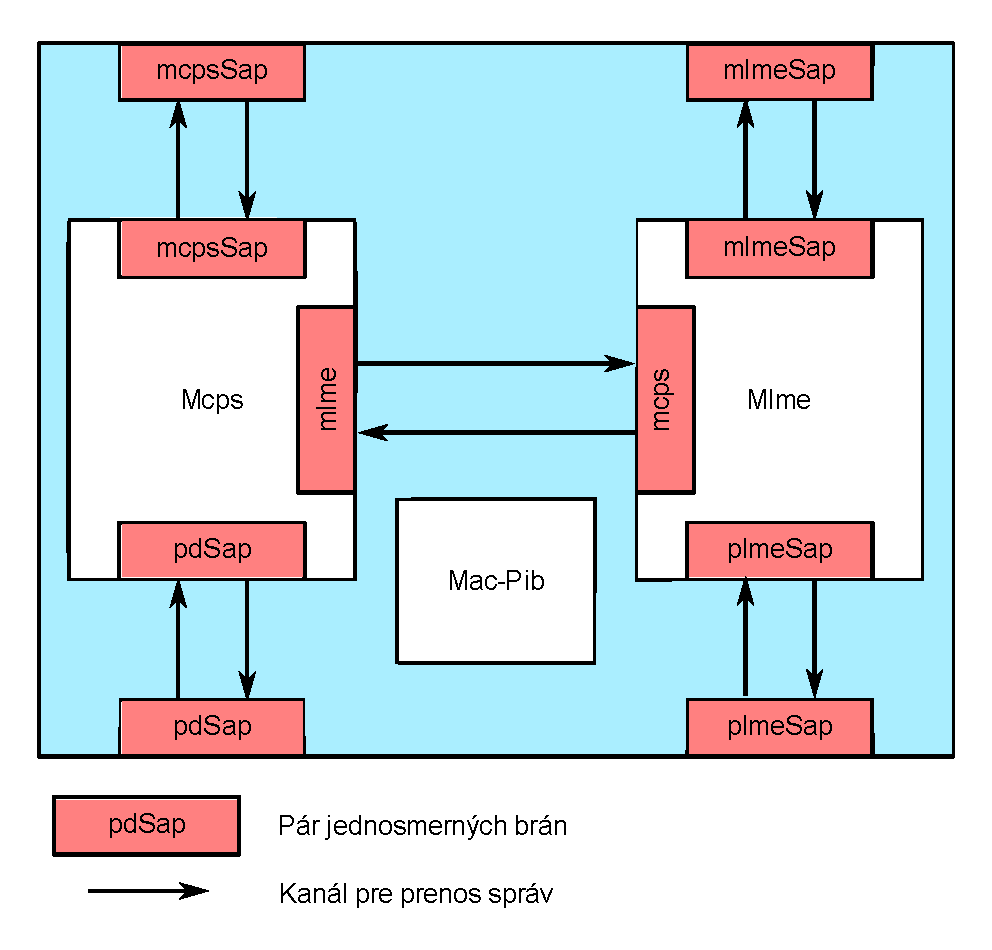
\includegraphics[width=120mm]{figures/architecture_mac}
\caption{Podoba implementovaného modelu linkovej vrstvy}
\label{fig:architecture_mac}
\end{center}
\end{figure}

\section{Fyzická vrstva - PHY}
\indent\indent Fyzická vrstva nášho modelu simuluje transformáciu bitov dodaných linkovou vrstvou na signál, ktorý je následne šírený médiom. Štandard pracuje so 7 komunikačnými módmi (obr. ~\ref{tab:frequencies}). Logika všetkých týchto módov je našim modelom podporovaná na strane komunikačných uzlov, ale pri začiatku simulácie sa musí nastaviť na jednu prenosovú frekvenciu \texttt{ChannelControl}. V tomto bude sa plánuje iný pohľad na správu spojení v simulátore MiXiM a tento nedostatok by sa mal odstrániť. Simulačný model by tam dovoľoval viacero aktívnych správcov spojení (moduly \texttt{ConnectionManager}). Úlohy fyzickej vrstvy sú alokované do 2 entít - analogicky ako aj v predošlých vrstvách: datovej (PD - PHY Data entity) a riadiacej (PLME - PHY Management Entity). Výs\-tupom smerom do éteru je bod služby RF-SAP a predstavuje rozhranie k rádiovému vysielaču/prijímaču.\\
\begin{figure}[htbp]
\begin{center}
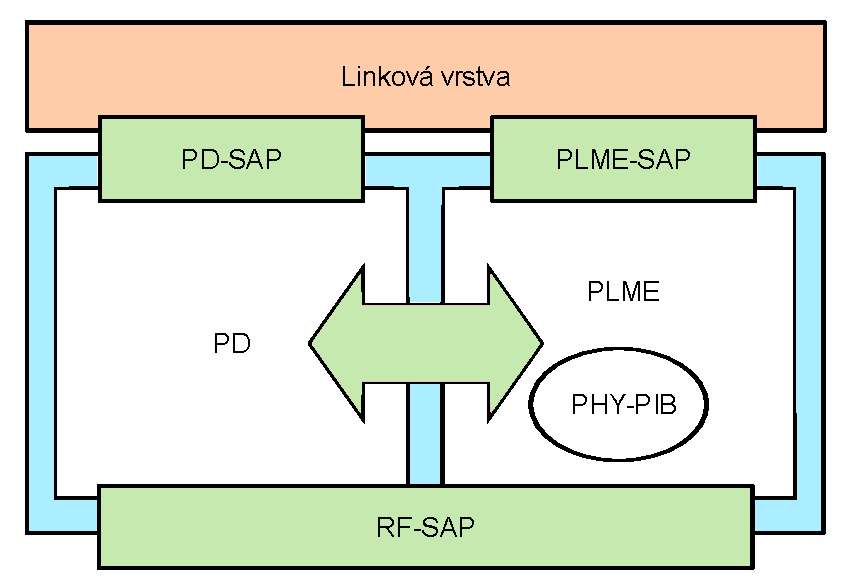
\includegraphics[width=120mm]{figures/topology_phy}
\caption{Referenčný model fyzickej vrstvy}
\label{fig:topology_phy}
\end{center}
\end{figure}
\subsection{Datová entita - PD}
\indent\indent Modul PD preposiela rámce medzi modulom \texttt{ChannelControl} a linkovou vrstvou cez bod prístupu PD-SAP. K rámcom pridáva dodatočné bity označované ako preamble a SFD bity (Starting Frame Delimiter). Tieto slúžia podľa špecifikácie k tomu, aby sa prijímací čip zosynchronizoval na týchto prijatých postupnostiach bitov. Vrstva PD nastavuje aj premennú \textit{lastMsgTimestamp}, ktorá je štruktúrou typu \textit{SimTime} a predstavuje časovú značku prijatých rámcov. Táto značka je nastavená až po prijatí bitov patriacich do preamble časti a SFD sekvencie. Názornejšie to vysvetľuje obr.~\ref{fig:frame_phy}.
\begin{figure}[htbp]
\begin{center}
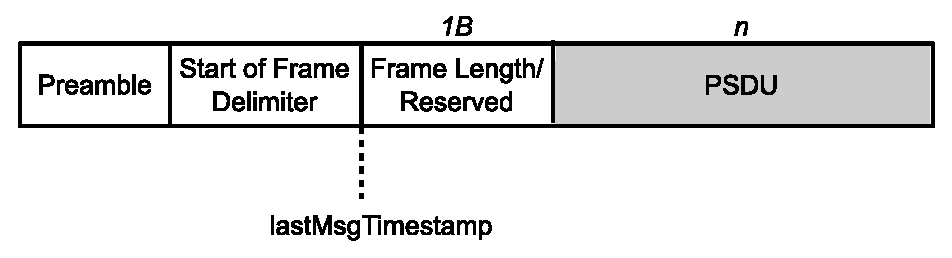
\includegraphics[width=140mm]{figures/frame_phy}
\caption{Spôsob enkapsulácie PSDU na fyzickej vrstve}
\label{fig:frame_phy}
\end{center}
\end{figure}
\paragraph{Implementácia}
Dĺžky polí preamble a SFD sa menia v závislosti od aktuálnej hodnoty \textit{phyCurrentChannel} a \textit{phyCurrentPage}. Sú zisťované priamo z modulu PHY-PIB (PHY layer Protocol Information Base). V tejto vrstve je to zatiaľ jediné miesto, kde je aktívne používaná utilita \texttt{Blackboard}. Pomocou nej sa vrstva PD dozvedá o tom, v akom stave je rádio a~aký je zámer MAC vrstvy (\textit{RX}/\textit{TX}). Podľa tejto informácie odosiela do bodu služby RF-SAP rámce.\\
\subsection{Riadiaca entita - PLME}
\indent\indent Riadiaca časť fyzickej vrstvy PLME má hlavne za úlohu spracovávať stavy rádia, prepínať ho na správnu frekvenciu a správny kanál. Úzko spolupracuje so sadou premenných a konštánt PHY-PIB. Vrstva ďalej informuje linkovú vrstvu o nameraných hodnotách pri ED (Energy Detection) snímaní okolia.\\
\paragraph{Implementácia}
Modul PLME je naprogramovaný tak, aby nedalo prípadnému záujemcovi veľa práce ho adaptovať na simulačný framework MiXiM. Tu sa nachádzajú úseky kódu, ktoré si budú vyžadovať úpravy k naplneniu cieľa. Jedná sa hlavne o zistenie spôsobu stavu energetickej hladiny kanálu. Tento údaj sa vysiela v primitíve PLME-ED-SCAN.confirm linkovej vrstve a v trochu inej podobe v primitíve PLME-CCA.confirm. V súvislosti s~ED skenovaním by bolo zaujímavé vedieť, aký je časový interval medzi prijatím správy PLME-ED-SCAN.request a odoslaním odpovede na ňu PLME-ED-SCAN.confirm. Pretože samotný údaj o dĺžke vykonávaného skenu je spracovaný linkovou vrstvou, ktorá o~tejto dĺžke neinformuje PLME modul, ale dovtedy opakuje vysielanie požiadavku na ED sken, dokedy jej nevyprší timer \textit{TIMER\_ED\_SCAN}. Následne modul MLME pracuje s~najvyššie zaznamenanou hodnotou vrátenou v správe PLME-ED-SCAN.confirm. Mimo to, modul PLME má za úlohu pristupovať do sady premenných a konštánt PHY-PIB za účelom predania ich hodnôt vyšším vrstvám cez primitívu PLME-GET.confirm, alebo ich nastavenia primitívou PLME-GET.request.\\
\indent Tento modul aj spracováva požiadavku pre vykonanie Clear Channel Assessment procedúry PLME-CCA.request. Za týmto účelom kontaktuje modul \texttt{SnrEval} a z neho vie zistiť, či je kanál v daný moment v stave \textit{IDLE}, alebo nie.\\
\begin{figure}[htbp]
\begin{center}
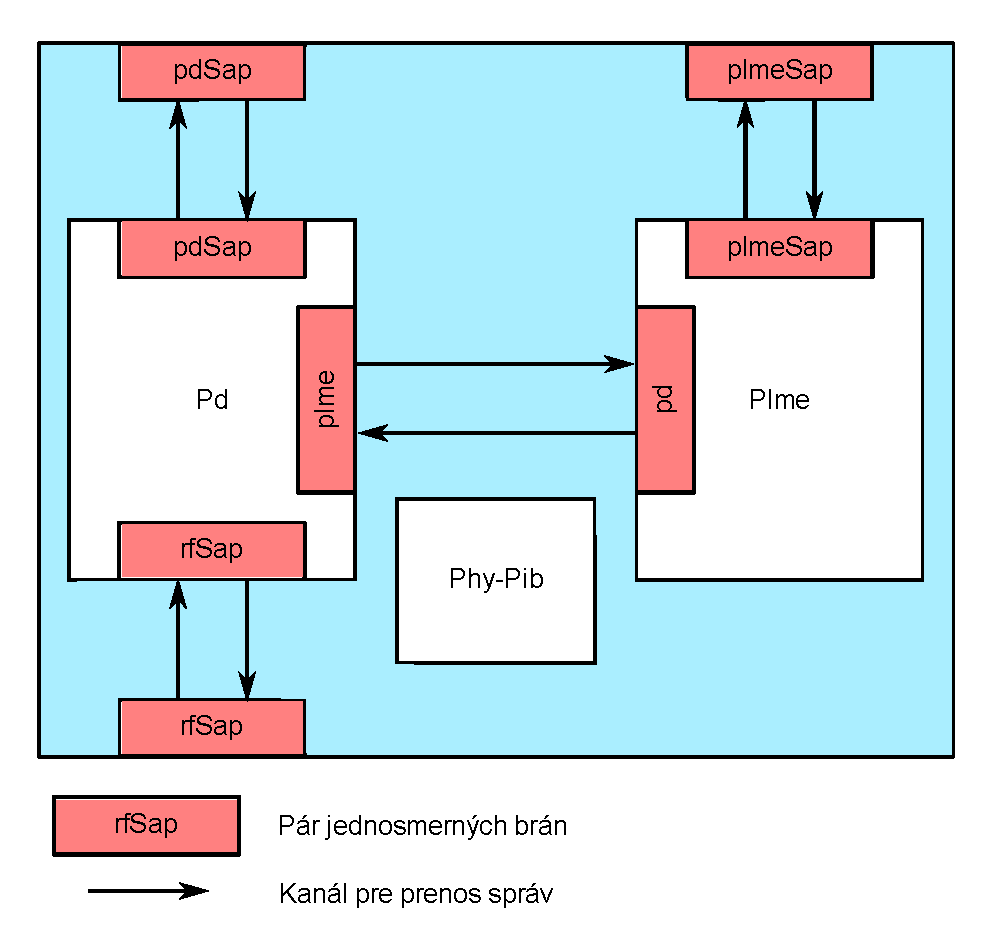
\includegraphics[width=120mm]{figures/architecture_phy}
\caption{Podoba implementovaného modelu fyzickej vrstvy}
\label{fig:architecture_phy}
\end{center}
\end{figure}
\subsection{Väzba na Mobility Framework}
\indent\indent Súčasťou fyzickej vrstvy v našom modeli sú už okrem spomenutých modulov aj moduly \texttt{SnrEval} a \texttt{SnrDecider}. Spôsob, akým zapadajú do architektúry modelu PHY je uvedený na obr.~\ref{fig:architecture_nic}. Tieto moduly sú súčasťou každej simulácie pod rozšírením Mobility Framework a v skutočnosti sú to upravené moduly z knižníc MF pre potreby nášho simulátora. Modul \texttt{SnrEval802154} vysiela rámce priamo modulu \texttt{ChannelControl}. V~opačnom smere, smere prijímania rámcov rozhoduje, či rámec sa príjme ako rámec, alebo je uvažovaný len ako príspevok k šumu. To závisí od toho, či je vypočítaná sila zaznamenaného signálu vyššia ako nastavená citlivosť prijímača. Energetická úroveň prijatého signálu sa počíta podľa vzorca$$P_{recv}=\frac{P_{send}\lambda^{2}}{16\pi^{2}l^{\alpha}}$$ kde $P_{send}$ znamená vyžarovací výkon, $\lambda$ vlnovú dĺžku nosnej, $\alpha$ predstavuje koeficient útlmu a $l$ vzdialenosť medzi zariadeniami. Modul \texttt{SnrEval802154} ďalej pracuje so stavom rádia a uverejňuje ho na \texttt{Blackboard}. V prípade spracovania správy ju pošle k modulu \texttt{SnrDecider802154}. Jeho úlohou je potom podľa úrovne SNR (Signal to Noise Ratio) a podľa prednastavenej hodnoty \textit{snrThreshold} prečítanej z modulu \texttt{ChannelControl} zistiť pravdepodobnosti chyby v prijatých rámcoch.\\
\indent Keď sa uvažuje vzduch ako spoločné prenosové médium, je potrebné si uvedomiť, že všetky zariadenia vzájomne sa ovplyvňujú. To znamená, že musia medzi nimi existovať spojenia. V prípade simulácie $n$ zariadení, počet spojení bude $n!$. Takýto prístup je pri svojom behu značne náročný na systémové prostriedky. V MF bola heuristickými metódami znížená táto náročnosť. Zadefinujme pojem interferenčná vzdialenosť. Jej hodnota bude predstavovať maximálnu prípustnú vzdialenosť medzi uzlami, pri ktorej ešte budeme uvažovať o ich vzájomnom rušení. Označme ju $r$. Vzdialenosť medzi uzlami označme $l$. Ak rozdelíme simulačnú plochu na štvorcové zóny s dĺžkou hrany $r$, môžme potom tvrdiť, že ovplyvňovať sa budú len uzly vrámci zóny a v vzájomne susediacich zónach. Uzly siete, ktoré sa nachádzajú vo vzdialenosti menšej, ako je interferenčná vzdialenosť ($l\in\langle0,r\rangle$), majú vytvorené medzi sebou spojenie. Uzly, ktoré sa nachádzajú vo vzdialenosti väčšej, ako je $2\sqrt{2}r$, spojenie určite vytvorené nemajú a~uzly, ktorých vzájomná vzdialenosť bude patriť do intervalu $l\in(r, 2\sqrt{2}r)$ budú mať spojenia vytvorené len v závislosti od ich polohy (viď obr.~\ref{fig:channelcontrol_areas}).\\
\indent Interferenčná vzdialenosť sa počíta podľa vzorca $$r=\left(\frac{\lambda^{2}P_{max}10^{3}}{16\pi^{2}10^{\frac{sat}{10}}}\right)^{\frac{1}{\alpha}}$$ kde $\lambda$ predstavuje vlnovú dĺžku nosnej frekvencie, $P_{max}$ najvyššiu hodnotu vyžarovacieho výkonu uzlu použitú v simulácii, premenná $sat$ hraničnú hodnotu útlmu (Signal Attenuation Threshold) a $\alpha$ koeficient útlmu. Pre nami použité hodnoty $\lambda=0,125$ ($f=2,4.10^{9}[Hz]$), $P_{max}=10\cdotp10^{-3}[mW]$, $sat=-112[dBm]$ a $\alpha=3,5$ vychádza hodnota interferenčnej vzdialenosti $r=219.555[m]$.\\
\indent V grafickom okne bežiacej simulácie (obr.~\ref{fig:screen_init} a obr.~\ref{fig:screen_beacons}) je dobre vidieť, aký výsledok sa dostaví s použitím uvedenej heuristiky pri pri nastavení prostredia podľa vyššie uvedených hodnôt parametrov. Spojenia sú vytvorené len medzi určitými uzlami a dynamicky vznikajú a zanikajú počas behu simulácie v závislosti na pohybe sieťových prvkov po ploche. V danom prípade bola nastavená dĺžka strany simulačného poľa o veľkosti $500m$.\\
\begin{figure}[htbp]
\begin{center}
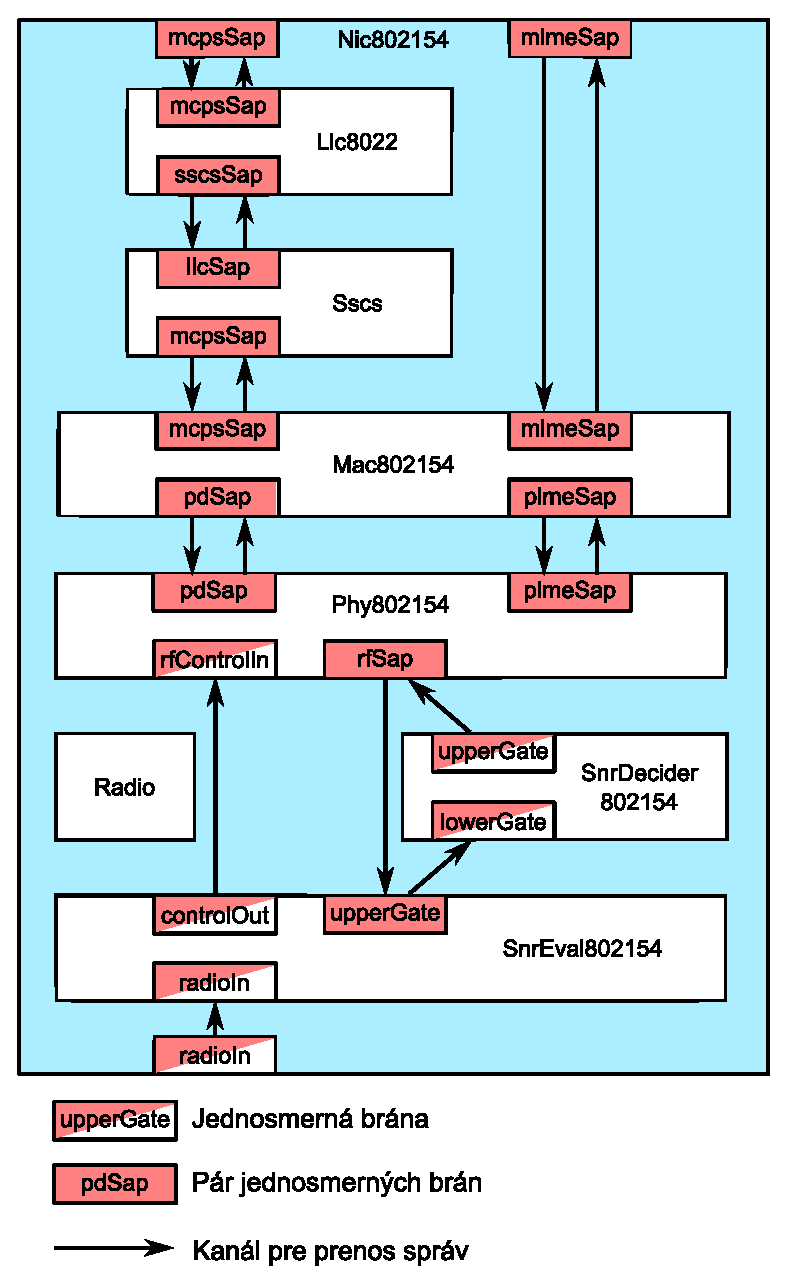
\includegraphics[width=120mm]{figures/architecture_nic}
\caption{Modul rozhrania 802.15.4 a jeho štruktúra v kontexte s rozšírením Mobility Framework}
\label{fig:architecture_nic}
\end{center}
\end{figure}

\section{Mobilita}
\indent\indent Mobility Framework poskytuje, ako už z jeho názvu vyplýva, silnú podporu mobilite modelov. V MF je mobilita rozdistribuovaná medzi všetky moduly FFD a RFD. Keďže nie je dôvod, aby jeden prvok ovplyvňoval druhý v pohybe, mobilita je počítaná na lokálnej úrovni jednotlivých prvkov. Informácia o vzájomných polohách zariadení je potom spracovávaná v module \texttt{SnrDecider} z informácii, ktoré poskytne \texttt{ChannelControl}. Mobility Framework 2.0 preview 3 má obsiahnutých niekoľko základných modelov pohybu po simulačnom poli. K základným patria:\\
\paragraph{CircleMobility} kde prvok opisuje trajektóriu v tvare kružnice s definovaným stredom, polomerom, rýchlosťou, počiatočným uhlom zvierajúcim sprievodiča s osou X (\textit{startAngle}) a periodicitou updatovania danej polohy. Obdobne pracuje aj model \textbf{RectangleMobility}, ktorý definuje pohyb po obdĺžniku.
\paragraph{ConstSpeedMobility} je mobilita, ktorá simuluje pohyb zariadenia smerom k náhodne definovaným cieľom s konštantnou rýchlosťou. Po dosiahnutí tohoto konkrétneho cieľa je ďalej zvolený iný, tiež náhodný.
\paragraph{LinearMobility} modeluje pohyb po poli s definovaným počiatočným stavom (súradnice, uhol pohybu voči osi X, rýchlosť a zrýchlenie). Smer pohybu prvku sa potom zmení len pri dosiahnutí okraja poľa, na ktorom prebieha simulácia, a to podľa pravidla uhol dopadu $=$ uhol odrazu.
\paragraph{MassMobility}~\cite{massmobility99} opisuje nasledovný spôsob pohybu po poli: prvok sa pohybuje priamo po priamke po dobu náhodne dlhého intervalu. Dĺžka toho intervalu je daná normálnym rozložením. Po uplynutí tohoto intervalu zmení smer pohybu o uhol, ktorého veľkosť je tiež náhodné číslo z normálneho rozloženia. Zároveň zmení v tomto bode aj rýchlosť na nejakú náhodnú veľkosť. Po náraze na hranicu simulačnej zóny sa odrazí pod rovnakým uhlom. Tento model hovorí o tom, že prvky majú moment zotrvačnosti a nemenia smer pohybu nárazovo. Východzie hodnoty sú $changeInterval = normal(5, 0.1) [s]$, $changeAngleBy = normal(0, 30) [deg]$ a $speed = normal(avgSpeed, 0.01) [m/s]$.
\paragraph{TurtleMobility} modul spracováva pohyb opísaný externýmn súborom vo formáte *.xml. Pohyb je nadefinovaný určitými blokmi úsekov, ktoré majú zadanú počiatočnú zmenu smeru, rýchlosť a číslo, koľko krát sa danú blok opakuje.\\ \\
\indent Mobility modely v MF sú aj schopné pracovať s externe definovanými modelmi mobility simulátora \textbf{ANSim}~\cite{ansim_report} a s modelmi mobility formátu \textbf{BonnMotion}~\cite{bonnmotion_report}. Všetko závisí na tom, aký spôsob mobility architektúry je definovaný v súboroch \texttt{FFD.ned} a~\texttt{RFD.ned}.\\
\indent V simulátore MiXiM bude obsiahnutý podobný prístup k riešeniu mobility prvkov. Tam bude existovať aj centrálny prvok riadiaci mobilitu a eventuelné kolízie prvkov \texttt{ObjectManager}. Predpokladá sa, že množstvo mobility modelov z MF bude implementované aj do MiXiM frameworku.\\

\section{IP over IEEE 802.15.4}
\indent\indent Až donedávna bola predstava, že IP prístup bude obchádzať LR-WPAN siete, pretože IP protokoly nebude možné preškálovať na linky s nízkymi prenosovými rýchlosťami, z~ktorých množstvo funguje v energeticky úsporných režimoch. IEEE 802.15.4 rámce sú relatívne malé a celý stack protokolov sa musí zmestiť do obmedzeného pamäťového priestoru. Návrh štandardu IETF 6LoWPAN pre IPv6 komunikáciu~\cite{rfc_4919} a~\cite{rfc_4944} cez IEEE 802.15.4 zmenil pohľad na danú problematiku. S podporou šifrovania AES-128 zahrnul základné bezpečnostné a autentizačné mechanizmy. Uvedený štandard definuje spôsob prenosu IP paketov cez siete štandardu IEEE 802.15.4 vďaka čomu umožňuje interoperabilitu medzi zariadeniami na rôznych linkách v hierarchii siete a zároveň dovoľuje paralelné fungovanie zariadení v týchto sieťach, ktoré nepoužívajú IP pakety k prenosu dát.\\
\indent Nasadenie IP technológie nad IEEE 802.15.4 má mnohé výhody. Menovite odpadá veľké množstvo potrebných smerovačov rôznych IEEE 802.15.4 protokolov, riadiacich a~bezpečnostných procedúr, pretože v týchto veciach sa môžme spoľahnúť na protokoly z rodiny TCP/IP. Nevýhodou nasadenia IPv6 sú veľké polia v hlavičke paketu a~spolu s~užitočným obsahom paketu presahujú prípustné veľkosti rámcov IEEE 802.15.4. 6LoWPAN formát v základnom režime pracuje s extrémne kompaktným záhlavím IP, ktoré rozširuje v prípade, že viaceré vlastnosti a schopnosti IPv6 protokolu sú využívané. Napríklad pri komunikácii susediacich 802.15.4 zariadení, polia obsahujúce IP adresy môžu byť skrátené takmer na nulu. V plnej forme sú použité v prípade, že jeden koniec komunikačného toku sa nachádza mimo 802.15.4 siete. Pri prekročení veľkosti MPDU, ktorú sú schopné zariadenia preniesť, sa pristupuje k fragmentácii. Tiež návrh 6LoWPAN dovoľuje smerovať rámce pomocou IP v sietiach LR-WPAN. Senzorové siete budú obsahovať brány (gateways), ktorých funkcionalita bude zredukovaná na úlohu jednoduchého smerovača medzi senzorovou a konvenčnou sieťou.\\
\begin{figure}[htbp]
\begin{center}
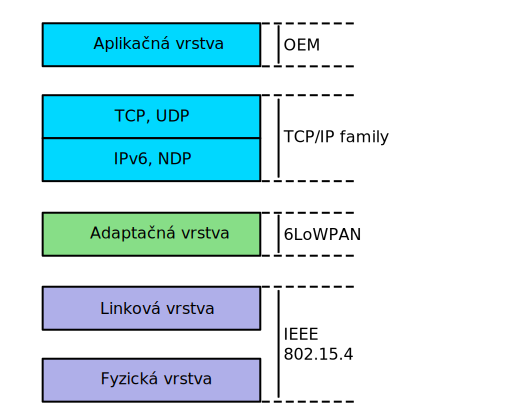
\includegraphics[width=120mm]{figures/ip_ieee}
\caption{Architektúra modulu komunikujúceho IP protokolmi na LR-WPAN sieti}
\label{fig:ip_ieee}
\end{center}
\end{figure}
\indent Pre nasadenie IP komunikácie je pripravené rozhranie na linkovej vrstve, ktoré poskytuje adaptačnej vrstve vstupné brány \texttt{input mlmeSapIn}, \texttt{input mcpsSapIn} a výstupné \texttt{output mlmeSapOut}, \texttt{output mcpsSapOut}. Modul linkovej vrstvy je implementovaný tak, aby korektne spracoval sekvencie správ pre inicializáciu siete (správy typu MLME-SCAN.request, MLME-SET.request, MLME-START.request, MLME-ASSOCIATE.request, MLME-BEACON-NOTIFY.indication). Tieto správy sú postačujúce na to, aby sa adaptačný modul nakonfiguroval pre správne prenášanie paketov IP, zviazal IPv6 s 64-bit IEEE adresami, alebo 16-bit krátkymi adresami a bol schopný enkapsulovať IP pakety do IEEE 802.15.4 rámcov. Presné definície správ, cez ktoré je možné naviazať adaptačnú vrstvu k linkovej vrstve sú uvedené v súbore \texttt{Messages.msg} s prefixom \texttt{Mlme}.


\cleardoublepage\chapter{Funkčnosť, výsledky testovania}

\indent\indent Na priloženom obrázku~\ref{fig:screen_init} je stav už nami pripravenej simulácie tak, ako ho zobrazuje grafické rozhranie OMNeT++. Pre názornosť bola mobilita aktivovaná len na prvku endDevice[0]. Ten sa počas behu simulácie stratí z dosahu zariadenia routerHost[2], čo je pekne vidieť na obr.~\ref{fig:screen_beacons}. Zobrazené linky znamenajú, že zariadenia sú ešte v dosahu svojich vyselačov, čo ale negarantuje spoľahlivý prenos dát medzi nimi.
\begin{figure}[htbp]
\begin{center}
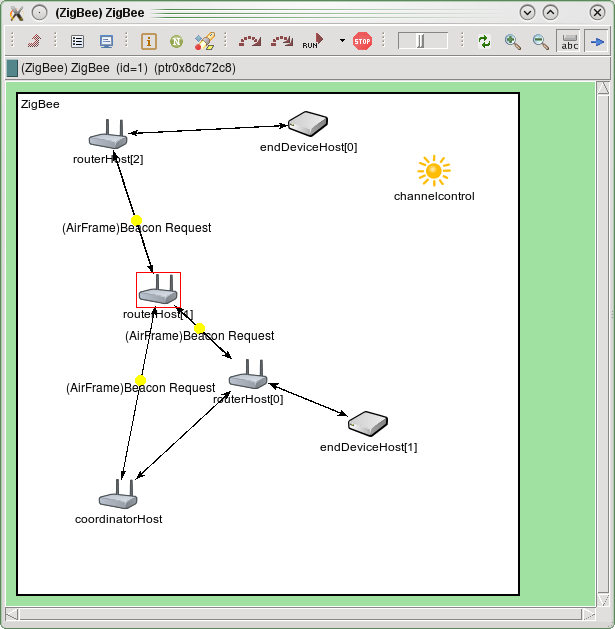
\includegraphics[width=100mm]{figures/screen_init}
\caption{Inicializovaná simulácia, modul routerHost[1] vykonáva aktívny sken okolia}
\label{fig:screen_init}
\end{center}
\end{figure}
\begin{figure}[htbp]
\begin{center}
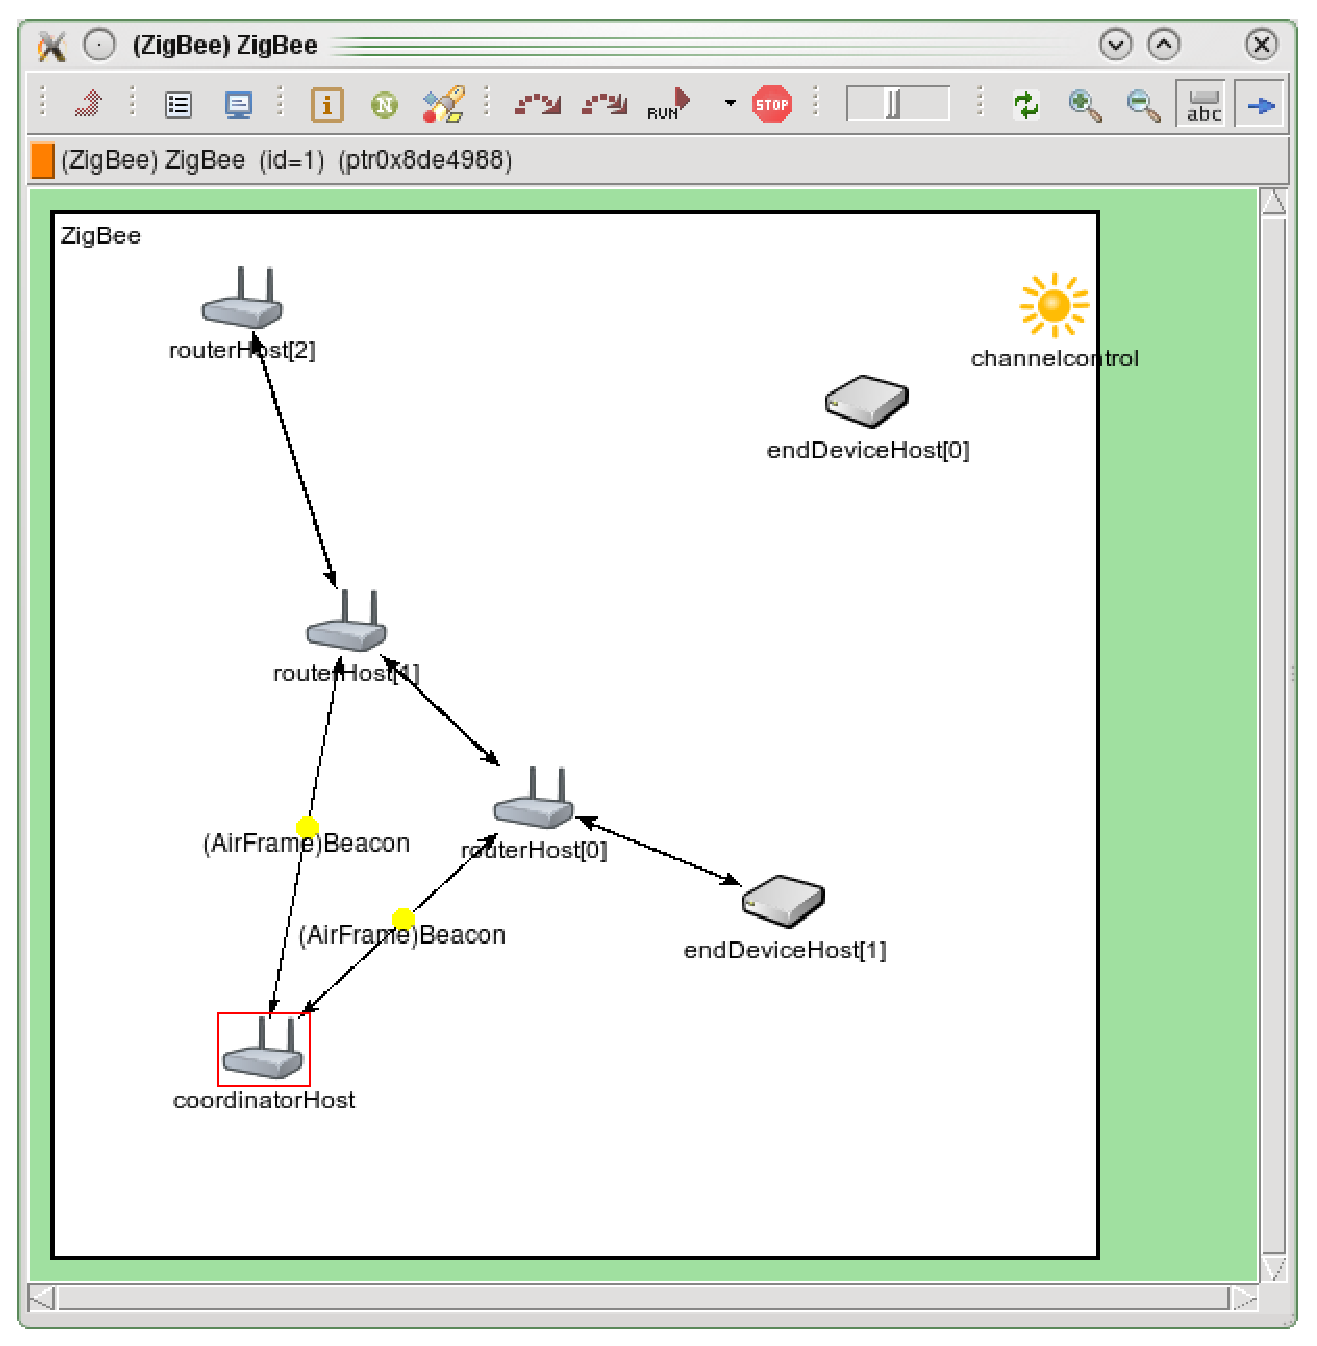
\includegraphics[width=100mm]{figures/screen_beacons}
\caption{Sieť vo svojej funkčnej konfigurácii, koordinátor vysiela beacon rámce zariadeniam v dosahu}
\label{fig:screen_beacons}
\end{center}
\end{figure}
\indent OMNeT++ ponúka veľmi efektívne nástroje na spracovávanie výsledkov simulácii. Jedným z nich je aj tzv. Event Log Viewer. Priebeh simulácie vrátane popisu zasielaných správ, stavov a ich väzba na simulačný čas sú zaznamenávané do súboru. Následne je možnosť tieto priebehy spracovať cez zásuvný modul v nástroji Eclipse, ktorý je dodávaný spolu so štvrtou hlavnou verziou simulátora. Takýmto spôsobom sú na nasledujúcich stranách tejto kapitoly vyobrazené a popísané niektoré zo základných implementovaných sekvencii z nášho modelu.\\
\indent Na prvom z uvedenej série~\ref{fig:chart_init} je sekvencia opisujúca úvodnú postupnosť správ pre vytvorenie siete PAN koordinátorom. Na sieťovej vrstve entitou {NLME je prijatá správa NLME-NETWORK-FORMATION.request, ktorej obsah definuje konfiguračné parametre siete, ktorú chceme vytvoriť. Podľa akceptovanej množiny kanálov sú spustené procedúry pre preskenovanie kanálov a zistenie ich energetických hladín. Pre každý kanál to predstavuje vykonanie série testov, z ktorých MLME vrstva si vyberie ten pesimistický variant. Po vykonaní daných analýz sa spustí tzv. aktívny sken na požadovaných kanáloch. Ten je doprevádzaný vysielaním požiadavku pre zaslanie beacon rámca. Po spracovaní výsledkov sa zapíšu konfiguračné premenné do informačných báz NWK-PIB a MAC-PIB a začína sa s rozposielaním beacon rámcov (obr.~\ref{fig:chart_beacon}) (v prípade, že sa jedná o beaconing mód). Na príslušnom obrázku je vidieť, že simulátor pracuje aj rýchlosťou šírenia signálu. To je ošetrené modulom \texttt{ChannelControl}. V prípade zvolenia vhodného kandidáta ako rodiča pre začlenenie sa do siete sa môže vyslať požiadavka pre asociáciu do siete. Táto správa je poslaná v CAP perióde. Na príslušnom grafe~\ref{fig:chart_associate_request} je možné spozorovať časovač CAP slot timer, ktorý určuje začiatok a koniec CAP slotov. Asso\-ciate Request Command požiadavok je posielaný (tak isto, ako iné riadiace správy) vždy na začiatku nového CAP slotu. Ďalej je daný obrázok zobrazuje posielanie potvrdzujúceho rámca (žiadosť o asociáciu vyžaduje potvrdzovanie), ktorý je iniciovaný v~MCPS vrstve cieľového zariadenia. Po uplynutí periódy o dĺžke \textit{macResponseWaitTime} symbolov môžme na sekvencii znázornenej na obr.~\ref{fig:chart_data_request} pozorovať transfer rámca typu Data Request Command z vrsvty MLME do vrstvy MCSP, ale aj keď už je obsiahnutý v~tejto fronte, čaká sa na začiatok nového CAP slotu (časovač CAP slot timer), ktorým sa vyšle PLME vrstve príkaz na vykonanie CCA procedúry. V prípade, že tá detekuje kanál v~stave \textit{IDLE}, je Data Request Command príkaz poslaný cieľu. Prijatie takéhoto rámca je tiež potvrdené ACK rámcom. Odpoveďou potom bude vyslanie Associate Response Command príkazu (obr.~\ref{fig:chart_associate_response}).\\
\indent Z dôvodu zjednodušenia modelu je možné v jeden okamih asociovať len jeden uzol. Každý ďalší požiadavok o asociáciu bude ignorovaný.\\
\begin{figure}[htbp]
\begin{center}
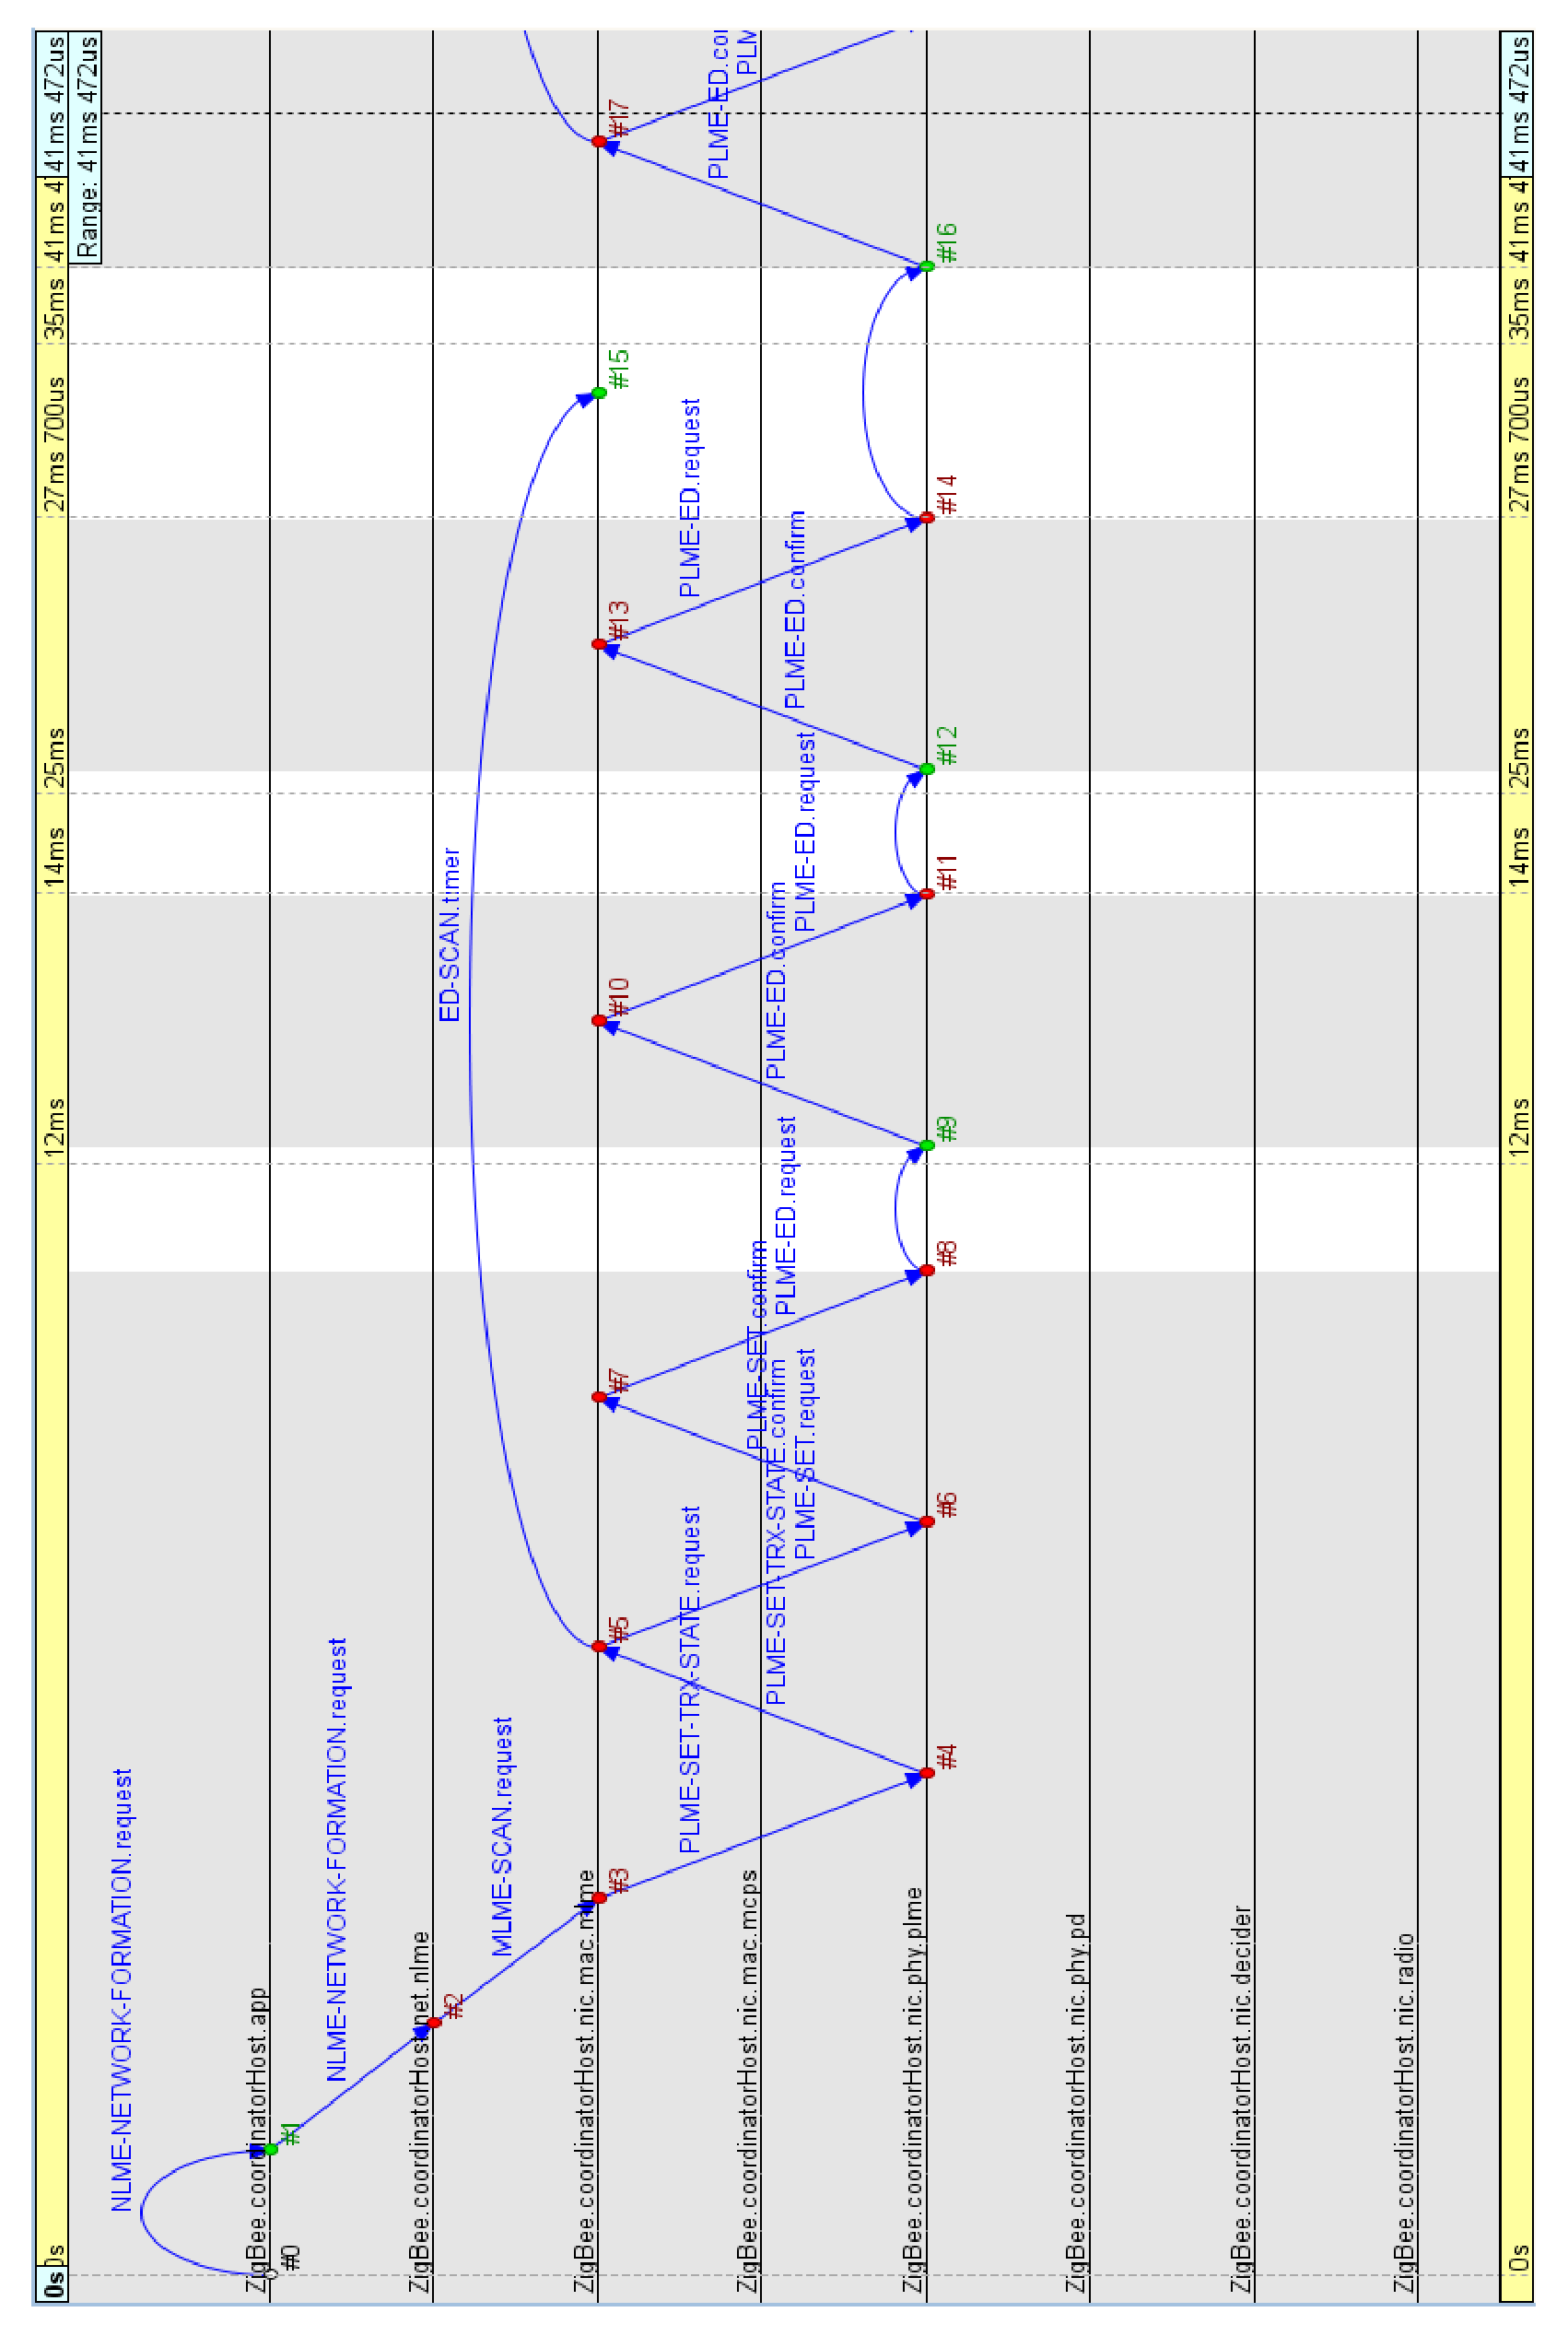
\includegraphics[width=140mm]{figures/chart_init}
\caption{Inicializácia koordinátora, ED sken}
\label{fig:chart_init}
\end{center}
\end{figure}
\begin{figure}[htbp]
\begin{center}
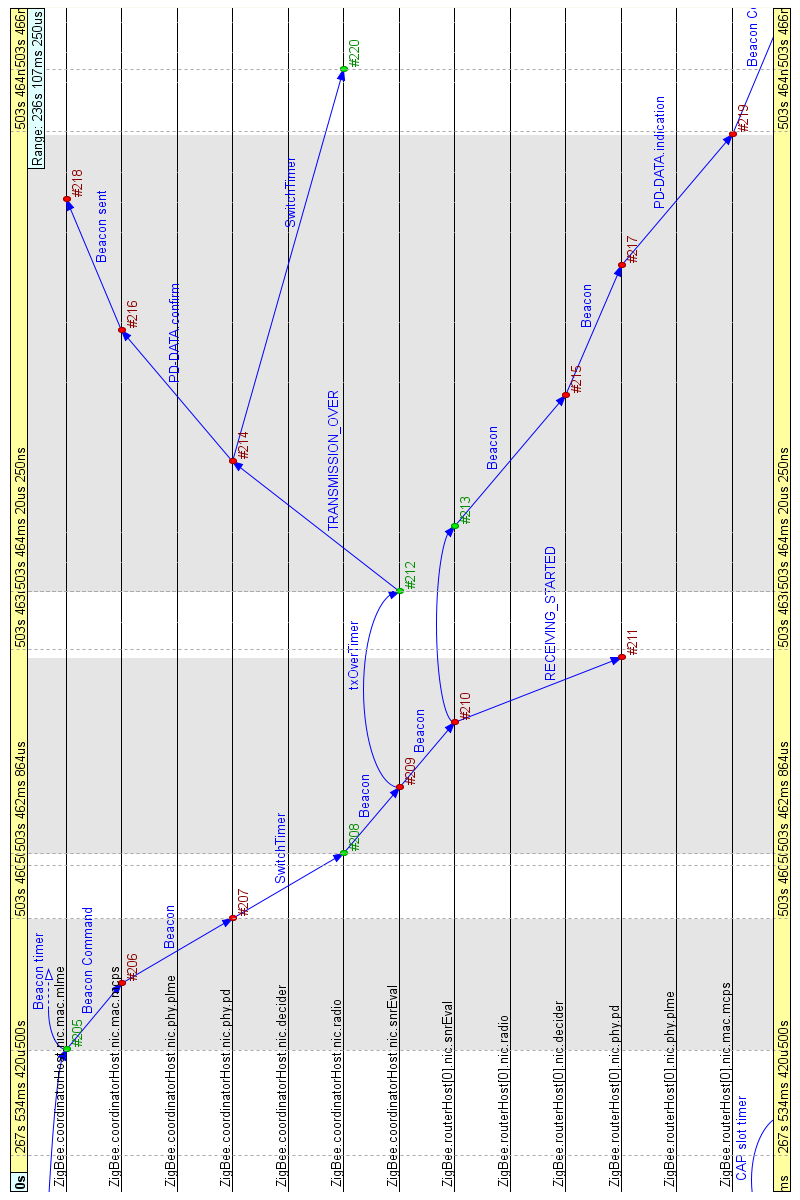
\includegraphics[width=140mm]{figures/chart_beacon}
\caption{Vysielanie a prijatie beacon rámcov}
\label{fig:chart_beacon}
\end{center}
\end{figure}
\begin{figure}[htbp]
\begin{center}
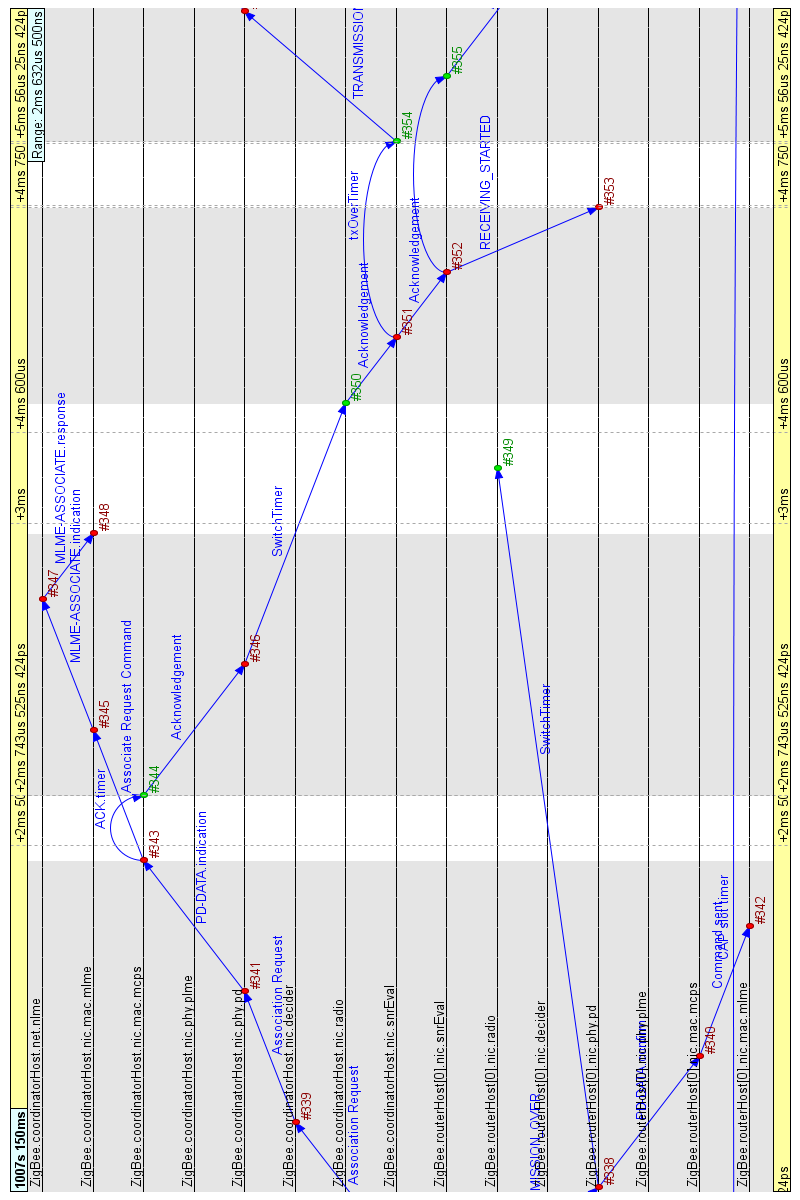
\includegraphics[width=140mm]{figures/chart_associate_request}
\caption{Spracovanie žiadosti o asociáciu}
\label{fig:chart_associate_request}
\end{center}
\end{figure}
\begin{figure}[htbp]
\begin{center}
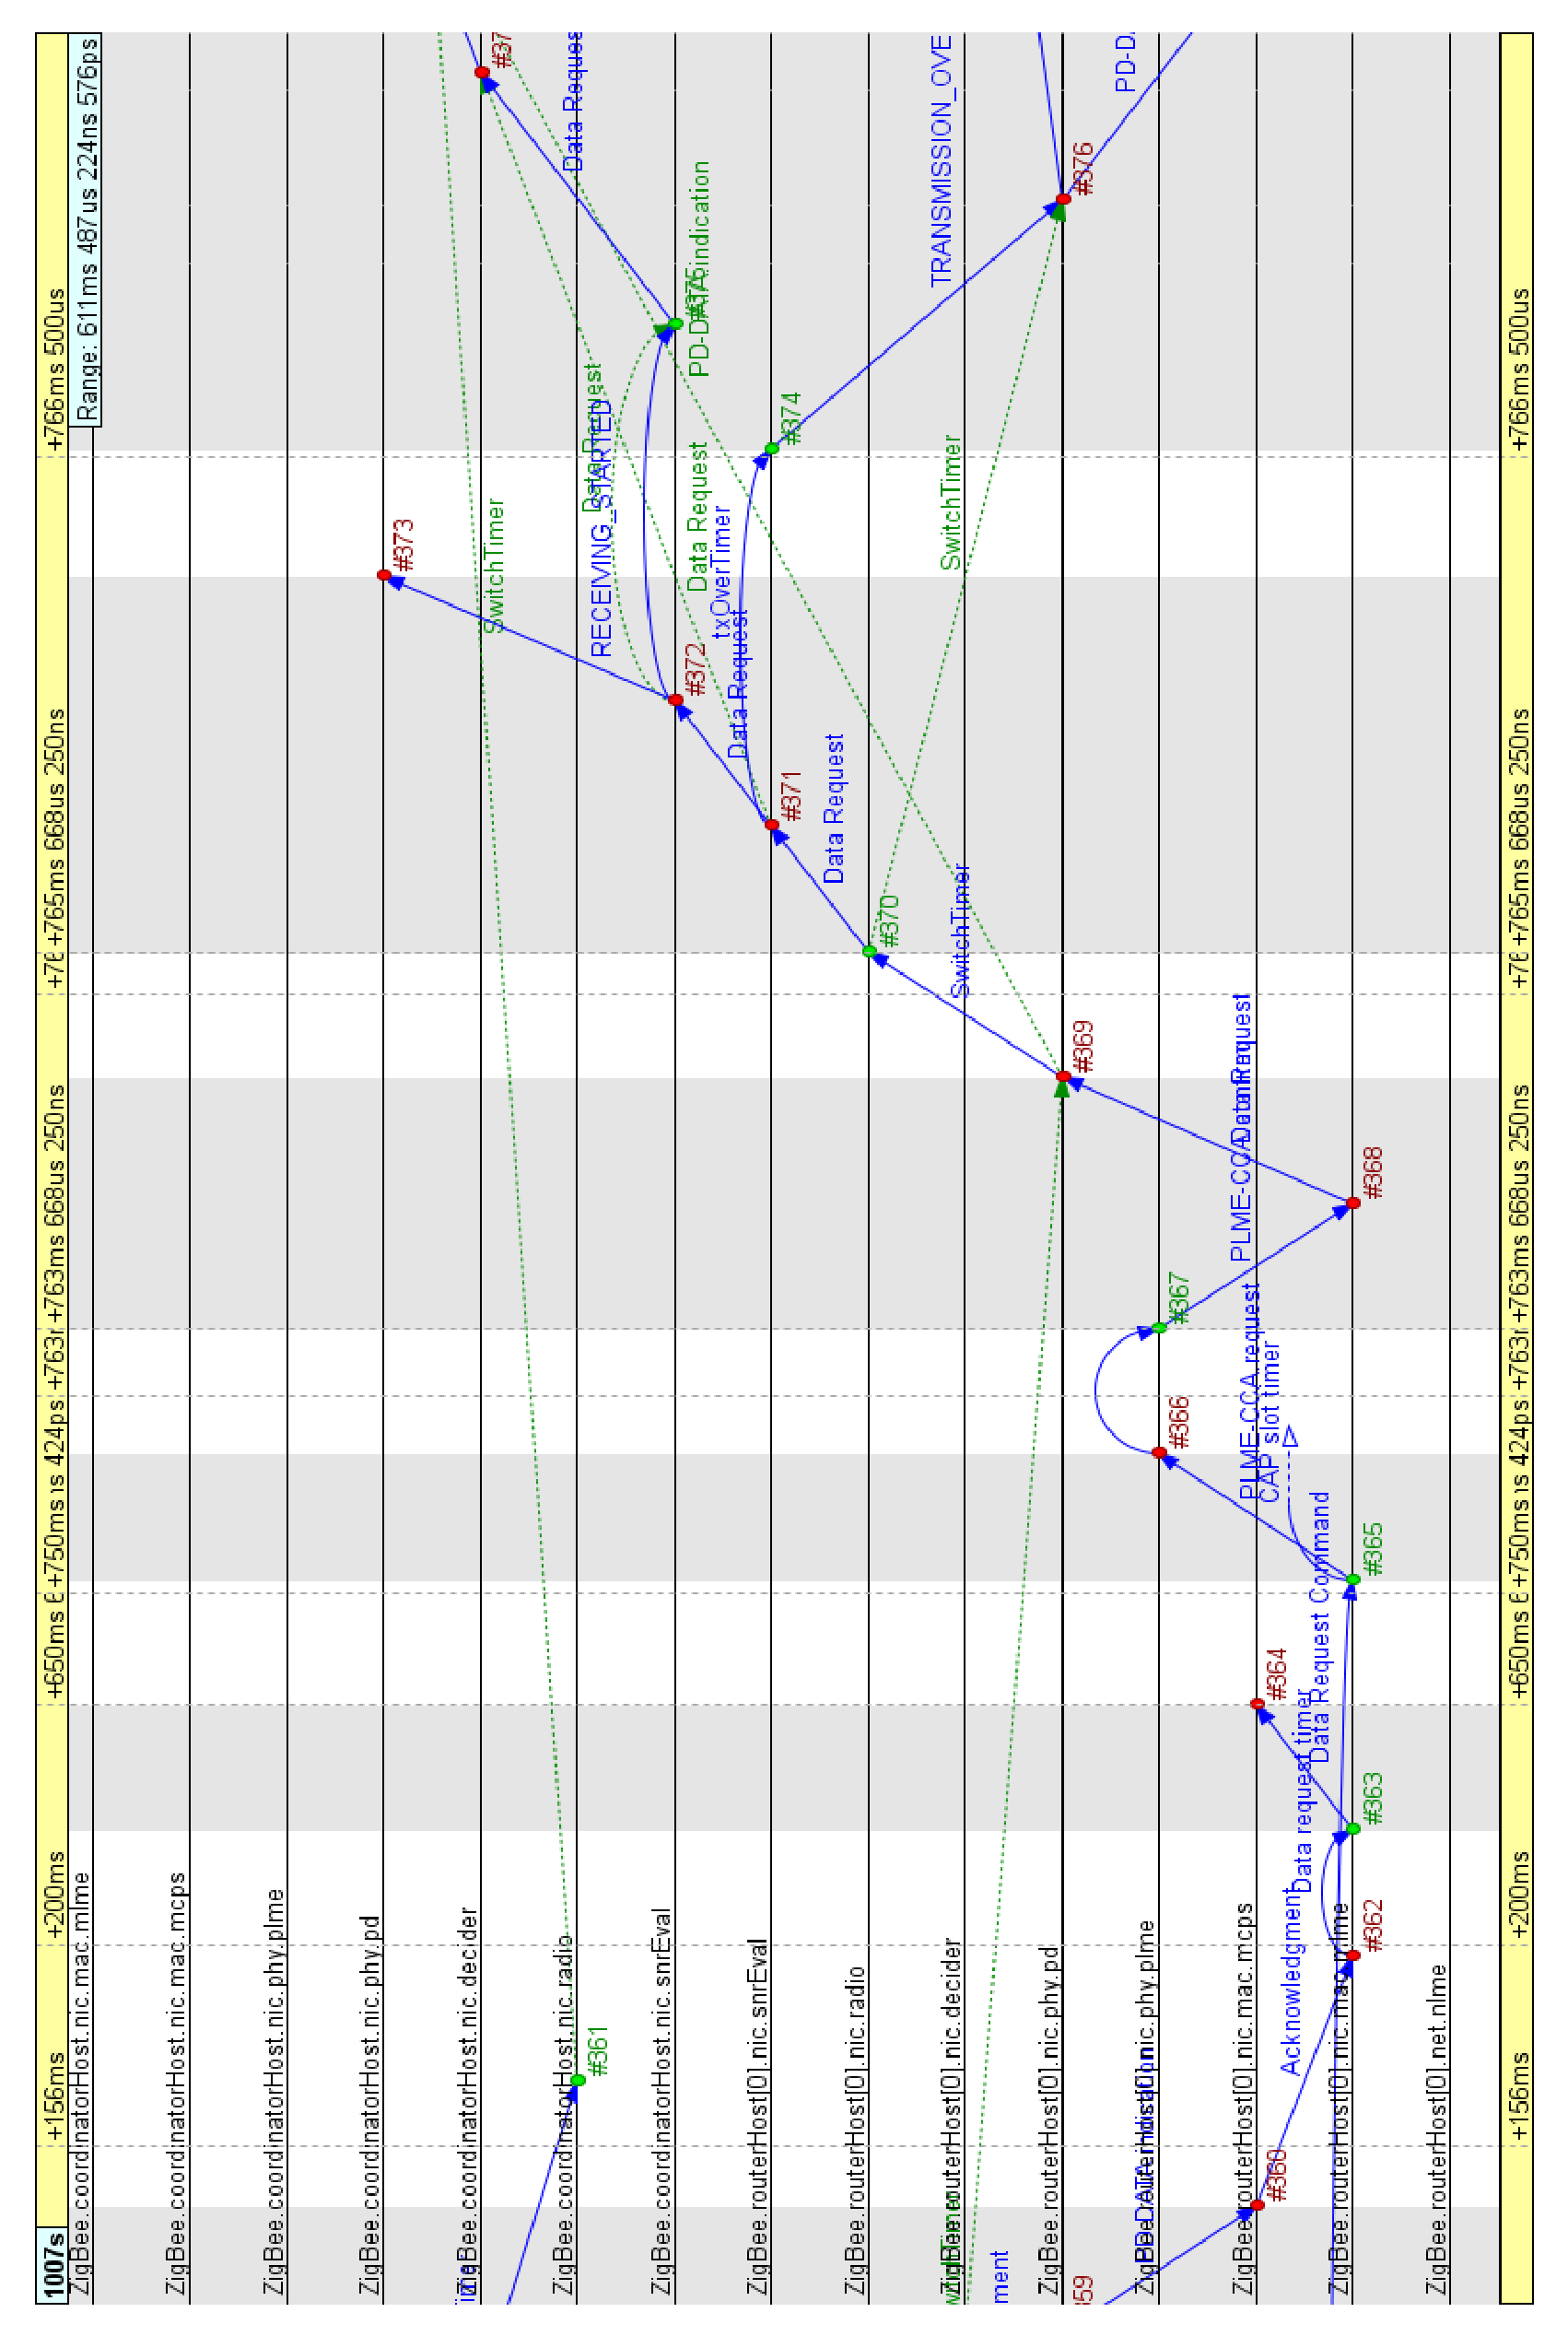
\includegraphics[width=140mm]{figures/chart_data_request}
\caption{Žiadosť o zaslanie dát, CCA procedúra}
\label{fig:chart_data_request}
\end{center}
\end{figure}
\begin{figure}[htbp]
\begin{center}
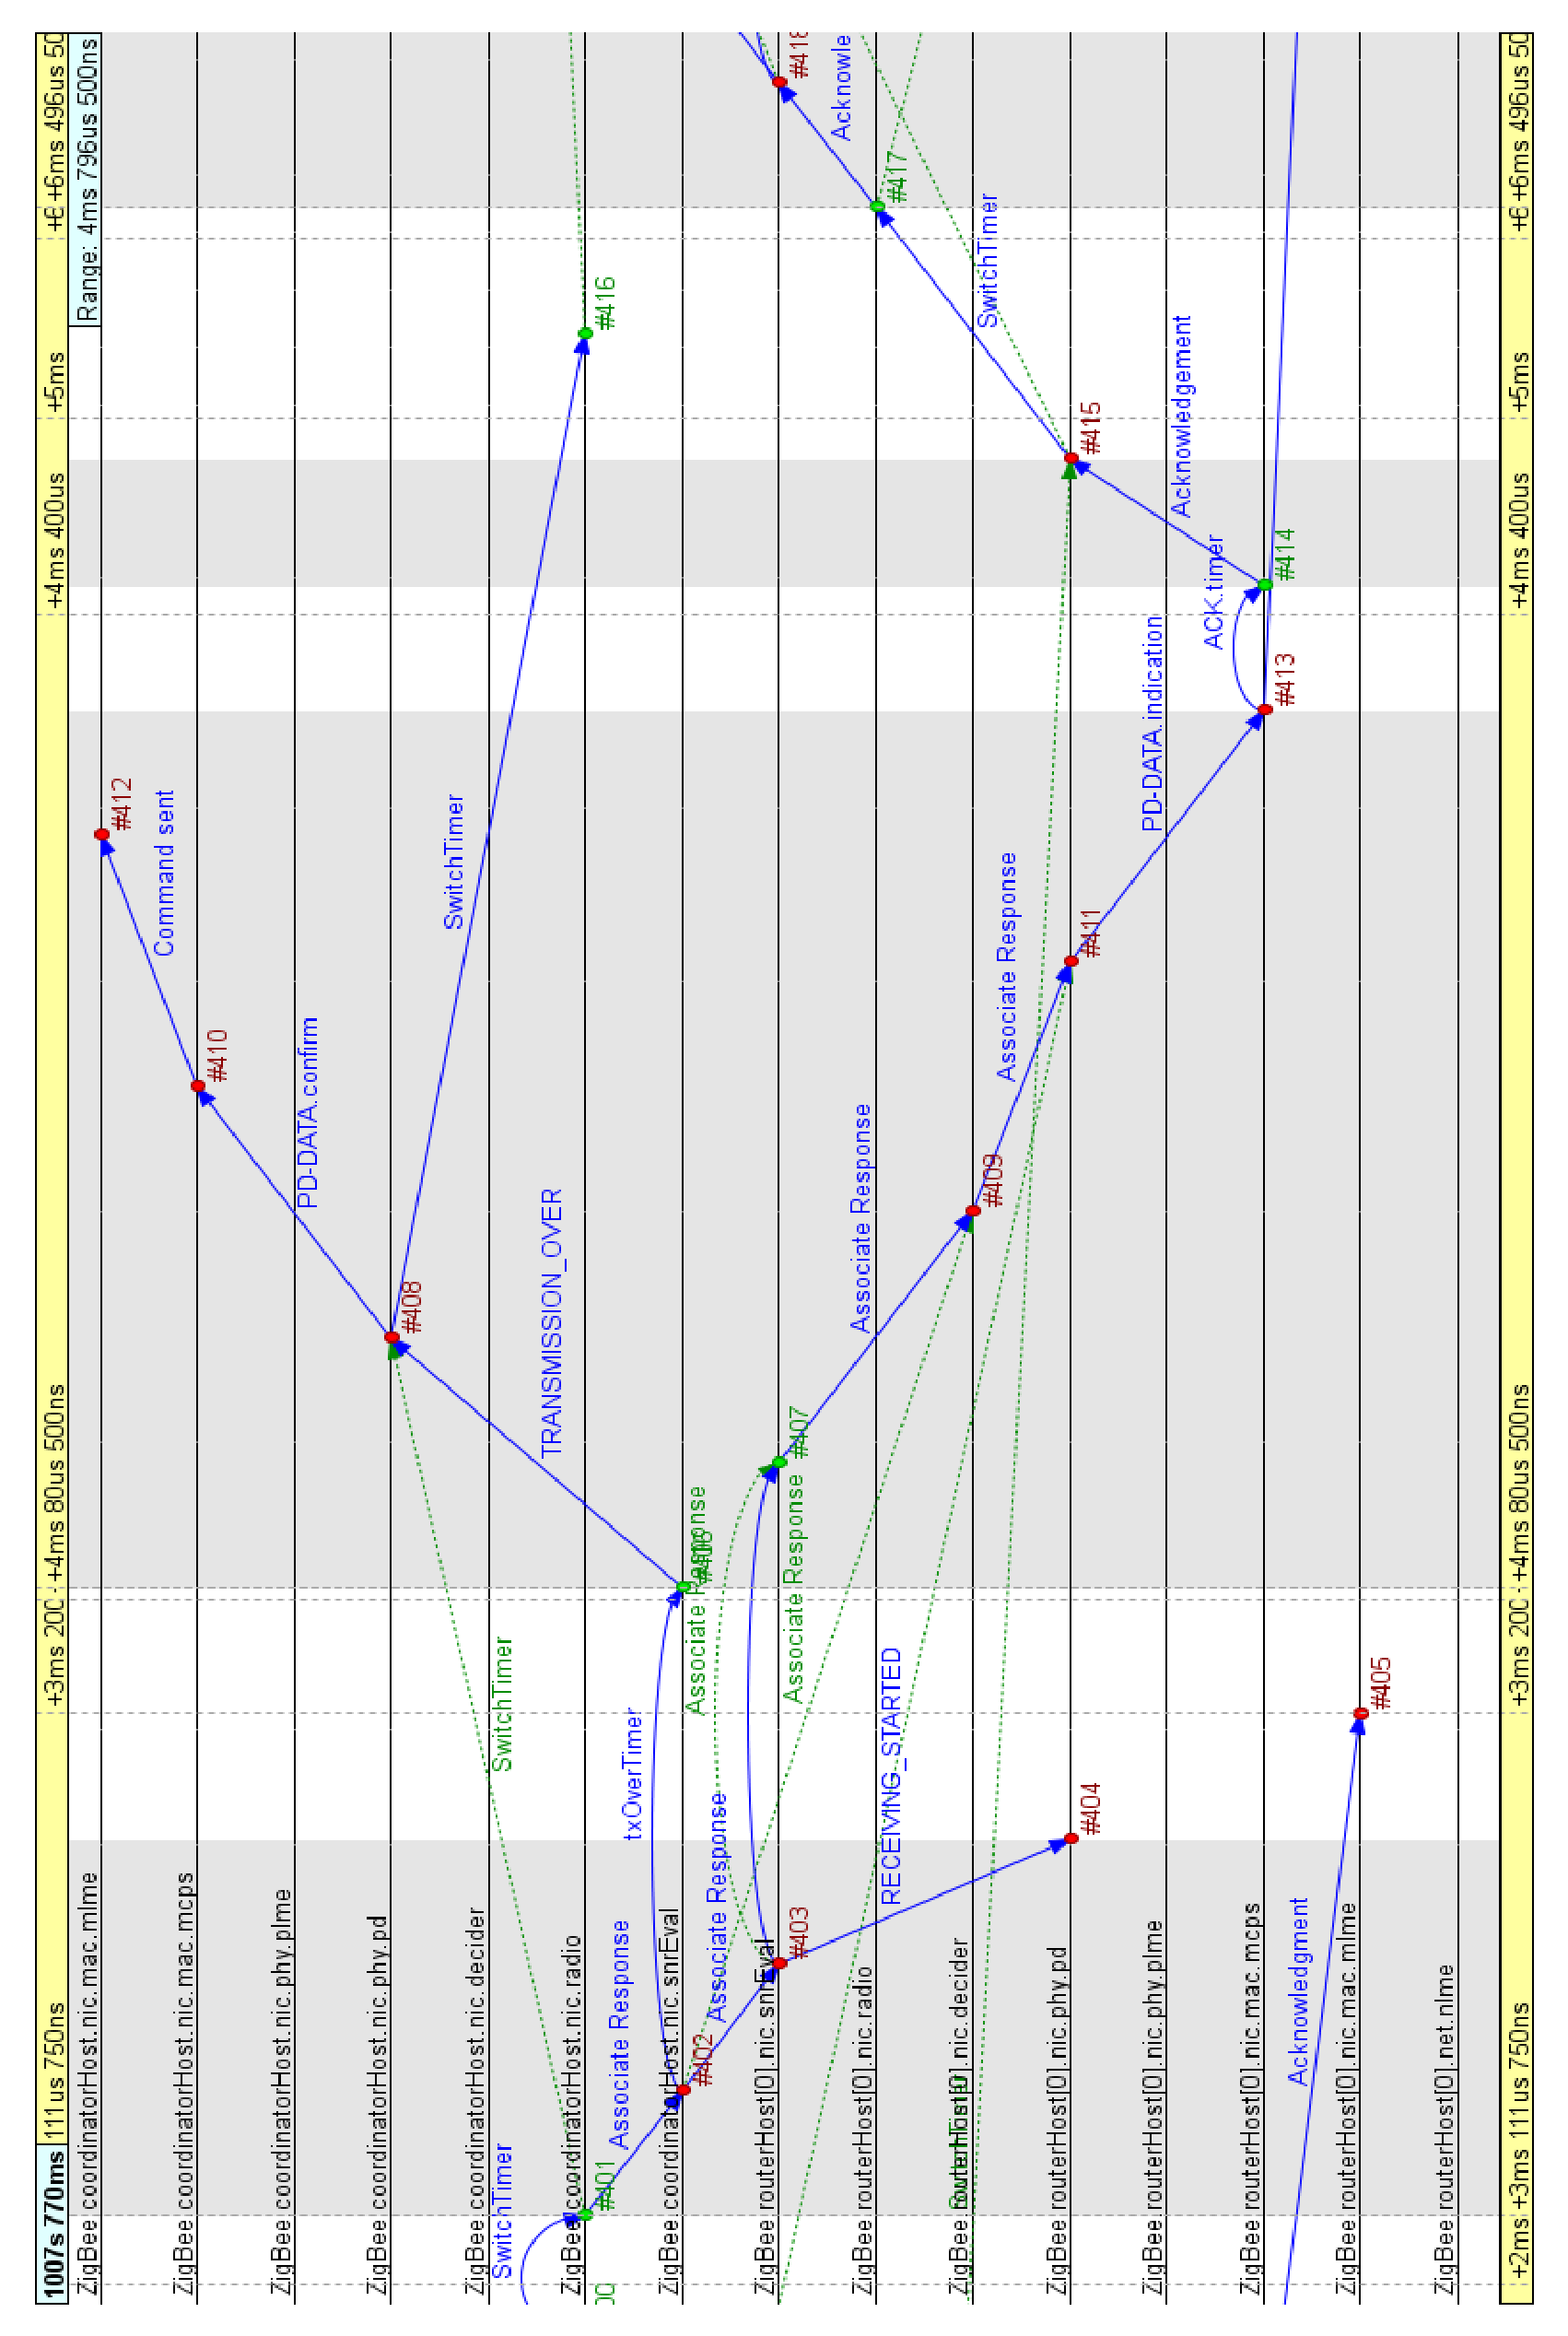
\includegraphics[width=140mm]{figures/chart_associate_response}
\caption{Odpoveď na žiadosť o asociáciu, jej spracovanie}
\label{fig:chart_associate_response}
\end{center}
\end{figure}

\cleardoublepage\chapter{Záver}
\indent\indent V práci sme prezentovali simulačný model sietí ZigBee a IEEE 802.15.4b-2006 navrhnutý v populárnom simulačnom nástroji OMNeT++. Mimo štruktúrovania jednotlivých uzlov podľa funkcionality na FFD a RFD, model implementuje podstatnú časť správy PAN siete, ako je definovaná v špecifikácii. V porovnaní s našim predchádzajúcim modelom siete IEEE 802.15.4-2003 definuje flexibilnejšiu štruktúru, je naviazaný na Mobility Framework a zároveň predpripravený pre nasadenie v prichádzajúcom simulačnom frameworku MiXiM. Mimo schopnosti vyhľadať sieť a asociovať sa do nej, pracuje model s CSMA-CA mechanizmom, vie si vytvárať a udržovať zoznamy susediacich prvkov a fungujúcich PAN sietí vo svojom okolí, vysielať a spracovávať beacon rámce a má predpripravené základné konštrukcie pre nasadenie GTS mechanizmu.\\
\indent Predstavený bol aj model prenosu IPv6 paketov sieťami LR-WPAN. Takéto využitie by sa ponúkalo napríklad v PDA zariadeniach.\\
\indent V prípadnej budúcej práci je priestor na dokončenie daného GTS mechanizmu, spracovanie osirotenia prvku, ktorý je úzko naviazaný na predstavené vlastni mobility nášho modelu a doplnenie vyšších vrstiev, hlavne sieťovej o smerovanie rámcov. Po implementácii týchto vlastností by bolo prospešné doplniť model o bezpečnostné procesy a pozorovať ich vplyv na prenosové a výkonové vlastnosti sietí ZigBee. Tiež sa ponúka využitie v simulátore MiXiM na testovanie vzájomného vplyvu s WiFi sieťami postavenými napríklad na nastupujúcom štandarde IEEE 802.11n.\\

%*****************************************************************************
% Seznam literatury je v samostatnem souboru reference.bib. Ten
% upravte dle vlastnich potreb, potom zpracujte (a do textu
% zapracujte) pomoci prikazu bibtex a nasledne pdflatex (nebo
% latex). Druhy z nich alespon 2x, aby se poresily odkazy.

\bibliographystyle{abbrv}
%bibliographystyle{plain}
%\bibliographystyle{psc}
{
%JZ: 11.12.2008 (Nekdo chce mit v techto ukazkovych odkazech take odkaz 
%JZ: na CSTeX, tak at to k necemu vypada...)
\def\CS{$\cal C\kern-0.1667em\lower.5ex\hbox{$\cal S$}\kern-0.075em $}
\bibliography{reference}
}

% M. Dušek radi:
%\bibliographystyle{alpha}
% kdy citace ma tvar [AutorRok] (napriklad [Cook97]). Sice to asi neni  podle ceske normy (BTW BibTeX stejne neodpovida ceske norme), ale je to nejprehlednejsi.

%*****************************************************************************

\appendix

\cleardoublepage\chapter{Zoznam použitých skratiek}

\begin{description}
\item[ACK] Acknownledgment
\item[APDU] Application level Protocol Data Unit
\item[APP] Application
\item[APS] Application Support Sublayer
\item[APSDE] Application Support Sublayer Data Entity
\item[APSME] Application Support Sublayer Management Entity
\item[CSMA-CA] Carrier Sense Multiple Access - Collision Avoidance
\item[ED] Energy Detection
\item[FCS] Frame Check Sequence
\item[FEC] Forward Error Correction
\item[FFD] Full Functionality Device
\item[GTS] Guaranteed Time Slot
\item[GUI] Graphical User Interface
\item[IDE] Integrated Development Environment
\item[IEEE] Institute of Electrical and Electronics Engineers
\item[IETF] Internet Engineering Task Force
\item[IP] Internet Protocol
\item[ISM] Industrial Scientific and Medical
\item[LLC] Logical Link Control
\item[LR-WPAN] Low-Rate Wireless Personal Area Network
\item[MAC] Medium Access Control
\item[MAC-PIB] Medium Access Control layer Protocol Information Base
\item[MCPS] MAC Common Part Sublayer
\item[MF] Mobility Framework
\item[MHz] Megahertz
\item[MIMO] Multiple In, Multiple Out
\item[MLME] MAC Sublayer Management Entity
\item[MSB] Most Significant Bit
\item[NET] Network
\item[NLDE] Network Layer Data Entity
\item[NLME] Network Layer Management Entity
\item[NPDU] Network level Protocol Data Unit
\item[NWK] Network
\item[NWK-PIB] Network layer Protocol Information Base
\item[OEM] Original Equipment Manufacturer
\item[OFDM] Orthogonal Frequency Division Multiplexing
\item[PAN] Personal Area Network
\item[PD] PHY Data
\item[PDA] Personal Digital Assistent
\item[PDU] Protocol Data Unit
\item[RFD] Reduced Functionality Device
\item[PHY] Physical
\item[PLME] PHY Layer Management Entity
\item[RSSI] Received Signal Strength Indication
\item[SAP] Service Access Point
\item[SAT] Signal Attenuation Threshold
\item[SFD] Starting Frame Delimiter
\item[SINR] Signal to Interference plus Noise Ratio
\item[SNR] Signal to Noise Ratio
\item[SSCS] Sublayer-Specific Convergence Sublayer
\item[TCP] Transmission Control Protocol
\item[UWB] Ultra-Wideband
\item[Wi-Fi] Wireless Fidelity
\item[WPAN] Wireless Personal Area Network
\item[WSN] Wireless Sensor Network
\item[ZDO] ZigBee Device Object
\end{description}

%*****************************************************************************
%\chapter{UML diagramy}


%*****************************************************************************
\chapter{Obsah priloženého CD}

\begin{figure}[h]
\begin{center}
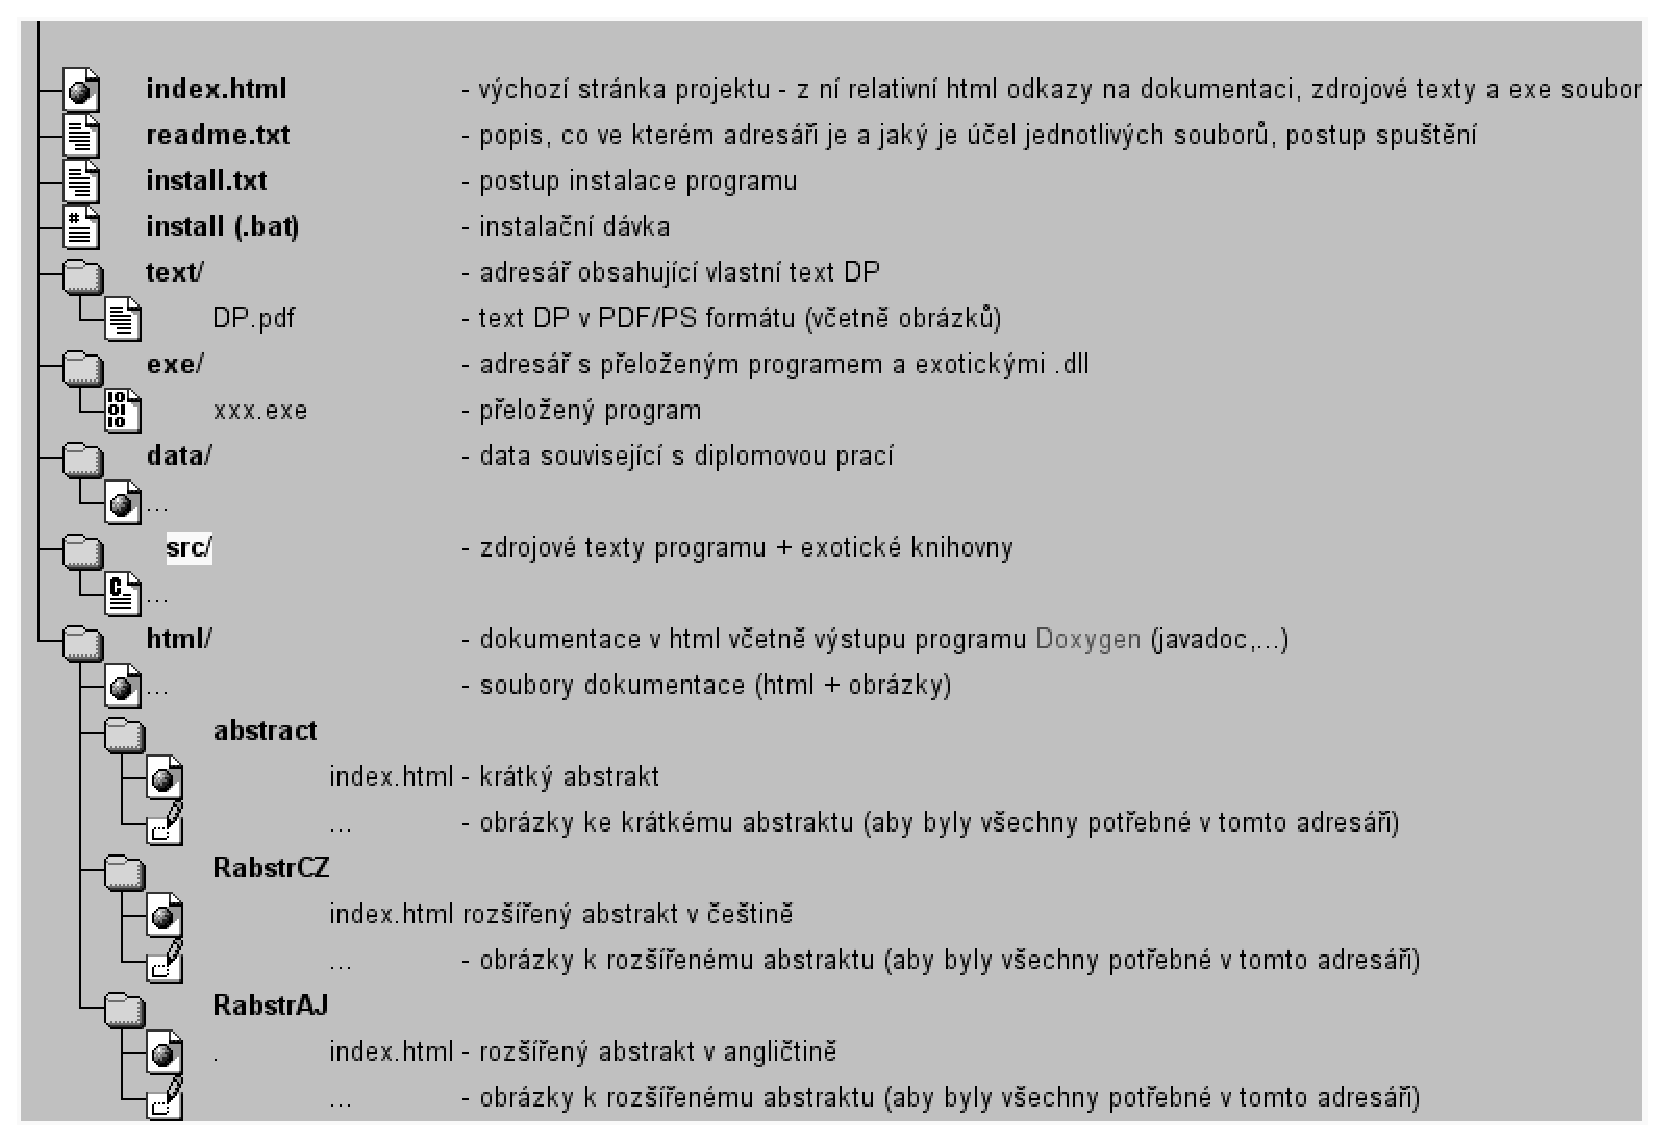
\includegraphics[width=14cm]{figures/seznamcd}
\caption{Obsah priloženého CD}
\label{fig:seznamcd}
\end{center}
\end{figure}
\end{document}
